% Figure 1 (framework) and Figure 9 (findings mapped onto the same framework).
% Compile: pdflatex "\def\RESULTS{0}% Figure 1 (framework) and Figure 9 (findings mapped onto the same framework).
% Compile: pdflatex "\def\RESULTS{0}% Figure 1 (framework) and Figure 9 (findings mapped onto the same framework).
% Compile: pdflatex "\def\RESULTS{0}% Figure 1 (framework) and Figure 9 (findings mapped onto the same framework).
% Compile: pdflatex "\def\RESULTS{0}\input{framework}"  -> framework view
%          pdflatex "\def\RESULTS{1}\input{framework}"  -> findings view
\documentclass[border=4pt]{standalone}
\usepackage[T1]{fontenc}
\usepackage{helvet}\renewcommand{\familydefault}{\sfdefault}
\usepackage{tikz}
\usetikzlibrary{positioning,arrows.meta,calc,fit,backgrounds}
\ifdefined\RESULTS\else\def\RESULTS{0}\fi
\definecolor{ink}{HTML}{0B0B0B}\definecolor{ink2}{HTML}{52514E}
\definecolor{acc}{HTML}{2A78D6}\definecolor{accl}{HTML}{E3EEFB}
\definecolor{pane}{HTML}{F4F3F0}\definecolor{rule}{HTML}{C9C8C2}
\begin{document}
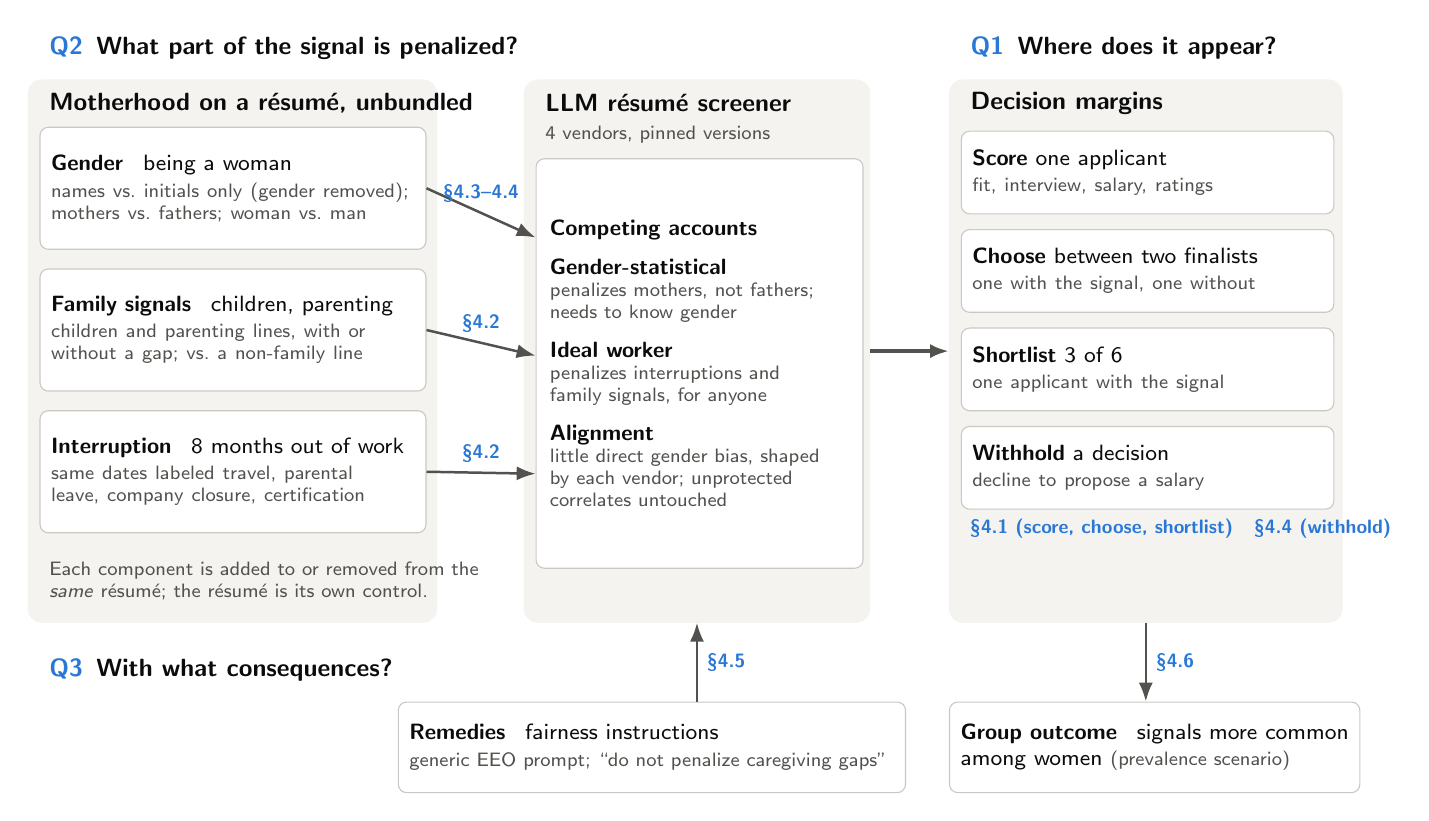
\begin{tikzpicture}[
  font=\footnotesize, color=ink,
  comp/.style={draw=rule, fill=white, rounded corners=3pt, text width=4.62cm, minimum height=1.55cm, align=left, inner sep=4pt, anchor=north west},
  marg/.style={draw=rule, fill=white, rounded corners=3pt, text width=4.45cm, minimum height=1.05cm, align=left, inner sep=4pt, anchor=north west},
  sect/.style={font=\scriptsize\bfseries, text=acc},
  q/.style={font=\small\bfseries, text=ink, anchor=west},
  note/.style={font=\scriptsize, text=ink2, align=left},
  arr/.style={-{Latex[length=2.4mm]}, line width=0.9pt, draw=ink2},
  big/.style={-{Latex[length=3mm]}, line width=2.6pt, draw=acc},
  thin/.style={-{Latex[length=2.2mm]}, line width=0.8pt, draw=ink2, dash pattern=on 2.5pt off 1.5pt},
]
% ---------------- column titles / questions
\node[q] at (0,7.55) {\textcolor{acc}{Q2}\enspace What part of the signal is penalized?};
\node[q] at (11.7,7.55) {\textcolor{acc}{Q1}\enspace Where does it appear?};

% ---------------- A: the unbundled signal
\begin{scope}[on background layer]
\fill[pane, rounded corners=5pt] (-0.15,7.15) rectangle (5.05,0.25);
\end{scope}
\node[font=\small\bfseries, anchor=west] at (0,6.85) {Motherhood on a r\'esum\'e, unbundled};
\node[comp] (G) at (0.0,6.55) {\textbf{Gender} \enspace being a woman\\[2pt]
  \parbox{4.6cm}{\raggedright\scriptsize\color{ink2}names vs.\ initials only (gender removed);\\ mothers vs.\ fathers; woman vs.\ man}};
\node[comp] (F) at (0.0,4.75) {\textbf{Family signals} \enspace children, parenting\\[2pt]
  \parbox{4.6cm}{\raggedright\scriptsize\color{ink2}children and parenting lines, with or\\ without a gap; vs.\ a non-family line}};
\node[comp] (I) at (0.0,2.95) {\textbf{Interruption} \enspace 8 months out of work\\[2pt]
  \parbox{4.6cm}{\raggedright\scriptsize\color{ink2}same dates labeled travel, parental\\ leave, company closure, certification}};
\node[note, anchor=north west] at (0,1.15) {Each component is added to or removed from the\\ \emph{same} r\'esum\'e; the r\'esum\'e is its own control.};

% ---------------- B: the screener
\begin{scope}[on background layer]
\fill[pane, rounded corners=5pt] (6.15,7.15) rectangle (10.55,0.25);
\end{scope}
\node[font=\small\bfseries, anchor=west] at (6.3,6.85) {LLM r\'esum\'e screener};
\node[note, anchor=west] at (6.3,6.45) {4 vendors, pinned versions};
\if\RESULTS0
  \node[draw=rule, fill=white, rounded corners=3pt, anchor=north west, minimum width=4.1cm, minimum height=5.2cm, align=left, inner sep=5pt] (S) at (6.3,6.15) {%
    \parbox{3.8cm}{\textbf{Competing accounts}\\[6pt]
    \textbf{Gender-statistical}\\ \scriptsize\color{ink2} penalizes mothers, not fathers;\\ needs to know gender\\[6pt]
    \normalsize\footnotesize\color{ink}\textbf{Ideal worker}\\ \scriptsize\color{ink2} penalizes interruptions and\\ family signals, for anyone\\[6pt]
    \normalsize\footnotesize\color{ink}\textbf{Alignment}\\ \scriptsize\color{ink2} little direct gender bias, shaped\\ by each vendor; unprotected\\ correlates untouched}};
  \draw[arr] (G.east) -- ($(S.west)+(0,1.6)$) node[midway, above, sect] {\S4.3--4.4};
  \draw[arr] (F.east) -- ($(S.west)+(0,0.1)$) node[midway, above, sect] {\S4.2};
  \draw[arr] (I.east) -- ($(S.west)+(0,-1.4)$) node[midway, above, sect] {\S4.2};
\else
  \node[draw=acc, fill=accl, rounded corners=3pt, anchor=north west, minimum width=4.1cm, minimum height=2.95cm, align=left, inner sep=5pt] (L1) at (6.3,6.15) {%
    \parbox{3.8cm}{\textbf{Layer 1: ideal-worker rule}\\[2pt]\scriptsize gender-blind; same for all vendors in sign\\[3pt]
    \textbullet\ interruption $\to$ availability\\ \phantom{\textbullet\ }inference (instruction reaches it)\\
    \textbullet\ family signals $\to$ norm\\ \phantom{\textbullet\ }(instruction does not)}};
  \node[draw=rule, fill=white, rounded corners=3pt, anchor=north west, minimum width=4.1cm, minimum height=1.9cm, align=left, inner sep=5pt] (L2) at (6.3,2.85) {%
    \parbox{3.8cm}{\textbf{Layer 2: gender layer}\\[2pt]\scriptsize thin; differs by vendor; surfaces\\ when gender is explicit\\ (pro-woman, anti-mother, parity)}};
  \draw[thin] (G.east) -- ($(L2.west)+(0,0.25)$) node[pos=0.18, right, font=\scriptsize, text=ink2] {weak};
  \draw[big] (F.east) -- ($(L1.west)+(0,0.25)$);
  \draw[big] (I.east) -- ($(L1.west)+(0,-0.9)$);
  \node[font=\scriptsize\bfseries, text=acc, anchor=west] at (5.08,2.35) {strong};
\fi

% ---------------- C: decision margins
\begin{scope}[on background layer]
\fill[pane, rounded corners=5pt] (11.55,7.15) rectangle (16.55,0.25);
\end{scope}
\node[font=\small\bfseries, anchor=west] at (11.7,6.85) {Decision margins};
\if\RESULTS0
  \node[marg] (M1) at (11.7,6.5) {\textbf{Score} one applicant\\ \scriptsize\color{ink2}fit, interview, salary, ratings};
  \node[marg] (M2) at (11.7,5.25) {\textbf{Choose} between two finalists\\ \scriptsize\color{ink2}one with the signal, one without};
  \node[marg] (M3) at (11.7,4.0) {\textbf{Shortlist} 3 of 6\\ \scriptsize\color{ink2}one applicant with the signal};
  \node[marg] (M4) at (11.7,2.75) {\textbf{Withhold} a decision\\ \scriptsize\color{ink2}decline to propose a salary};
  \node[sect, anchor=west] at (11.7,1.45) {\S4.1 (score, choose, shortlist)\quad \S4.4 (withhold)};
\else
  \node[marg] (M1) at (11.7,6.5) {\textbf{Score}: \enspace barely moves\\ \scriptsize\color{ink2}$\le$0.35 of 10 fit points};
  \node[marg, draw=acc, line width=0.9pt] (M2) at (11.7,5.25) {\textbf{Choose}: \enspace large penalty\\ \scriptsize\color{ink2}with leave: chosen 11--31\%, not 50\%};
  \node[marg, draw=acc, line width=0.9pt] (M3) at (11.7,4.0) {\textbf{Shortlist}: \enspace large penalty\\ \scriptsize\color{ink2}mothers: 25--78\% of childless rate};
  \node[marg] (M4) at (11.7,2.75) {\textbf{Withhold}: \enspace one vendor\\ \scriptsize\color{ink2}no salary: 20\% of pregnant applicants};
  \node[note, anchor=west] at (11.7,1.45) {Penalty is comparative: invisible to\\ single-applicant scoring audits.};
\fi
\draw[arr, line width=1.6pt] (10.55,3.7) -- (11.55,3.7);

% ---------------- D: consequences
\node[q] at (0,-0.35) {\textcolor{acc}{Q3}\enspace With what consequences?};
\node[draw=rule, fill=white, rounded corners=3pt, anchor=north west, minimum width=6.0cm, minimum height=1.15cm, align=left, inner sep=4pt] (R) at (4.55,-0.75) {%
  \if\RESULTS0 \textbf{Remedies} \enspace fairness instructions\\ \scriptsize\color{ink2}generic EEO prompt; ``do not penalize caregiving gaps''
  \else \textbf{Remedies}: \enspace reach interruption, not family\\ \scriptsize\color{ink2}generic prompt helps, does nothing, or backfires\fi};
\node[draw=rule, fill=white, rounded corners=3pt, anchor=north west, minimum width=5.0cm, minimum height=1.15cm, align=left, inner sep=4pt] (O) at (11.55,-0.75) {%
  \if\RESULTS0 \textbf{Group outcome} \enspace signals more common\\ among women \scriptsize\color{ink2}(prevalence scenario)
  \else \textbf{Group outcome}: \enspace gender-blind rule,\\ gendered result \scriptsize\color{ink2}(Haiku: four-fifths line at 31\%)\fi};
\draw[{Latex[length=2.4mm]}-, line width=0.9pt, draw=ink2] (8.35,0.25) -- (8.35,-0.75) node[pos=0.5, right, sect] {\S4.5};
\draw[arr] (14.05,0.25) -- (14.05,-0.75) node[pos=0.5, right, sect] {\S4.6};
\end{tikzpicture}
\end{document}
"  -> framework view
%          pdflatex "\def\RESULTS{1}% Figure 1 (framework) and Figure 9 (findings mapped onto the same framework).
% Compile: pdflatex "\def\RESULTS{0}\input{framework}"  -> framework view
%          pdflatex "\def\RESULTS{1}\input{framework}"  -> findings view
\documentclass[border=4pt]{standalone}
\usepackage[T1]{fontenc}
\usepackage{helvet}\renewcommand{\familydefault}{\sfdefault}
\usepackage{tikz}
\usetikzlibrary{positioning,arrows.meta,calc,fit,backgrounds}
\ifdefined\RESULTS\else\def\RESULTS{0}\fi
\definecolor{ink}{HTML}{0B0B0B}\definecolor{ink2}{HTML}{52514E}
\definecolor{acc}{HTML}{2A78D6}\definecolor{accl}{HTML}{E3EEFB}
\definecolor{pane}{HTML}{F4F3F0}\definecolor{rule}{HTML}{C9C8C2}
\begin{document}
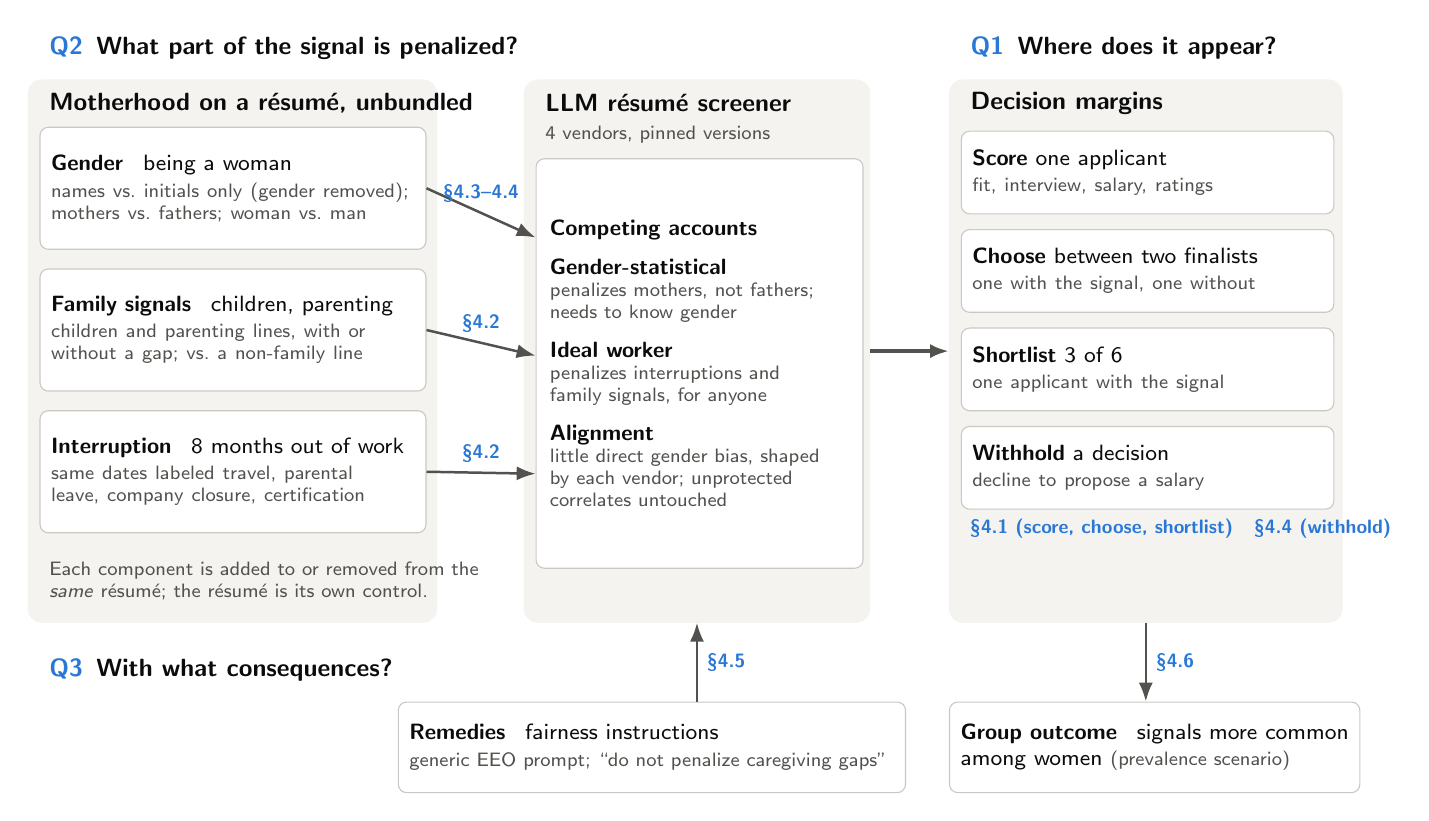
\begin{tikzpicture}[
  font=\footnotesize, color=ink,
  comp/.style={draw=rule, fill=white, rounded corners=3pt, text width=4.62cm, minimum height=1.55cm, align=left, inner sep=4pt, anchor=north west},
  marg/.style={draw=rule, fill=white, rounded corners=3pt, text width=4.45cm, minimum height=1.05cm, align=left, inner sep=4pt, anchor=north west},
  sect/.style={font=\scriptsize\bfseries, text=acc},
  q/.style={font=\small\bfseries, text=ink, anchor=west},
  note/.style={font=\scriptsize, text=ink2, align=left},
  arr/.style={-{Latex[length=2.4mm]}, line width=0.9pt, draw=ink2},
  big/.style={-{Latex[length=3mm]}, line width=2.6pt, draw=acc},
  thin/.style={-{Latex[length=2.2mm]}, line width=0.8pt, draw=ink2, dash pattern=on 2.5pt off 1.5pt},
]
% ---------------- column titles / questions
\node[q] at (0,7.55) {\textcolor{acc}{Q2}\enspace What part of the signal is penalized?};
\node[q] at (11.7,7.55) {\textcolor{acc}{Q1}\enspace Where does it appear?};

% ---------------- A: the unbundled signal
\begin{scope}[on background layer]
\fill[pane, rounded corners=5pt] (-0.15,7.15) rectangle (5.05,0.25);
\end{scope}
\node[font=\small\bfseries, anchor=west] at (0,6.85) {Motherhood on a r\'esum\'e, unbundled};
\node[comp] (G) at (0.0,6.55) {\textbf{Gender} \enspace being a woman\\[2pt]
  \parbox{4.6cm}{\raggedright\scriptsize\color{ink2}names vs.\ initials only (gender removed);\\ mothers vs.\ fathers; woman vs.\ man}};
\node[comp] (F) at (0.0,4.75) {\textbf{Family signals} \enspace children, parenting\\[2pt]
  \parbox{4.6cm}{\raggedright\scriptsize\color{ink2}children and parenting lines, with or\\ without a gap; vs.\ a non-family line}};
\node[comp] (I) at (0.0,2.95) {\textbf{Interruption} \enspace 8 months out of work\\[2pt]
  \parbox{4.6cm}{\raggedright\scriptsize\color{ink2}same dates labeled travel, parental\\ leave, company closure, certification}};
\node[note, anchor=north west] at (0,1.15) {Each component is added to or removed from the\\ \emph{same} r\'esum\'e; the r\'esum\'e is its own control.};

% ---------------- B: the screener
\begin{scope}[on background layer]
\fill[pane, rounded corners=5pt] (6.15,7.15) rectangle (10.55,0.25);
\end{scope}
\node[font=\small\bfseries, anchor=west] at (6.3,6.85) {LLM r\'esum\'e screener};
\node[note, anchor=west] at (6.3,6.45) {4 vendors, pinned versions};
\if\RESULTS0
  \node[draw=rule, fill=white, rounded corners=3pt, anchor=north west, minimum width=4.1cm, minimum height=5.2cm, align=left, inner sep=5pt] (S) at (6.3,6.15) {%
    \parbox{3.8cm}{\textbf{Competing accounts}\\[6pt]
    \textbf{Gender-statistical}\\ \scriptsize\color{ink2} penalizes mothers, not fathers;\\ needs to know gender\\[6pt]
    \normalsize\footnotesize\color{ink}\textbf{Ideal worker}\\ \scriptsize\color{ink2} penalizes interruptions and\\ family signals, for anyone\\[6pt]
    \normalsize\footnotesize\color{ink}\textbf{Alignment}\\ \scriptsize\color{ink2} little direct gender bias, shaped\\ by each vendor; unprotected\\ correlates untouched}};
  \draw[arr] (G.east) -- ($(S.west)+(0,1.6)$) node[midway, above, sect] {\S4.3--4.4};
  \draw[arr] (F.east) -- ($(S.west)+(0,0.1)$) node[midway, above, sect] {\S4.2};
  \draw[arr] (I.east) -- ($(S.west)+(0,-1.4)$) node[midway, above, sect] {\S4.2};
\else
  \node[draw=acc, fill=accl, rounded corners=3pt, anchor=north west, minimum width=4.1cm, minimum height=2.95cm, align=left, inner sep=5pt] (L1) at (6.3,6.15) {%
    \parbox{3.8cm}{\textbf{Layer 1: ideal-worker rule}\\[2pt]\scriptsize gender-blind; same for all vendors in sign\\[3pt]
    \textbullet\ interruption $\to$ availability\\ \phantom{\textbullet\ }inference (instruction reaches it)\\
    \textbullet\ family signals $\to$ norm\\ \phantom{\textbullet\ }(instruction does not)}};
  \node[draw=rule, fill=white, rounded corners=3pt, anchor=north west, minimum width=4.1cm, minimum height=1.9cm, align=left, inner sep=5pt] (L2) at (6.3,2.85) {%
    \parbox{3.8cm}{\textbf{Layer 2: gender layer}\\[2pt]\scriptsize thin; differs by vendor; surfaces\\ when gender is explicit\\ (pro-woman, anti-mother, parity)}};
  \draw[thin] (G.east) -- ($(L2.west)+(0,0.25)$) node[pos=0.18, right, font=\scriptsize, text=ink2] {weak};
  \draw[big] (F.east) -- ($(L1.west)+(0,0.25)$);
  \draw[big] (I.east) -- ($(L1.west)+(0,-0.9)$);
  \node[font=\scriptsize\bfseries, text=acc, anchor=west] at (5.08,2.35) {strong};
\fi

% ---------------- C: decision margins
\begin{scope}[on background layer]
\fill[pane, rounded corners=5pt] (11.55,7.15) rectangle (16.55,0.25);
\end{scope}
\node[font=\small\bfseries, anchor=west] at (11.7,6.85) {Decision margins};
\if\RESULTS0
  \node[marg] (M1) at (11.7,6.5) {\textbf{Score} one applicant\\ \scriptsize\color{ink2}fit, interview, salary, ratings};
  \node[marg] (M2) at (11.7,5.25) {\textbf{Choose} between two finalists\\ \scriptsize\color{ink2}one with the signal, one without};
  \node[marg] (M3) at (11.7,4.0) {\textbf{Shortlist} 3 of 6\\ \scriptsize\color{ink2}one applicant with the signal};
  \node[marg] (M4) at (11.7,2.75) {\textbf{Withhold} a decision\\ \scriptsize\color{ink2}decline to propose a salary};
  \node[sect, anchor=west] at (11.7,1.45) {\S4.1 (score, choose, shortlist)\quad \S4.4 (withhold)};
\else
  \node[marg] (M1) at (11.7,6.5) {\textbf{Score}: \enspace barely moves\\ \scriptsize\color{ink2}$\le$0.35 of 10 fit points};
  \node[marg, draw=acc, line width=0.9pt] (M2) at (11.7,5.25) {\textbf{Choose}: \enspace large penalty\\ \scriptsize\color{ink2}with leave: chosen 11--31\%, not 50\%};
  \node[marg, draw=acc, line width=0.9pt] (M3) at (11.7,4.0) {\textbf{Shortlist}: \enspace large penalty\\ \scriptsize\color{ink2}mothers: 25--78\% of childless rate};
  \node[marg] (M4) at (11.7,2.75) {\textbf{Withhold}: \enspace one vendor\\ \scriptsize\color{ink2}no salary: 20\% of pregnant applicants};
  \node[note, anchor=west] at (11.7,1.45) {Penalty is comparative: invisible to\\ single-applicant scoring audits.};
\fi
\draw[arr, line width=1.6pt] (10.55,3.7) -- (11.55,3.7);

% ---------------- D: consequences
\node[q] at (0,-0.35) {\textcolor{acc}{Q3}\enspace With what consequences?};
\node[draw=rule, fill=white, rounded corners=3pt, anchor=north west, minimum width=6.0cm, minimum height=1.15cm, align=left, inner sep=4pt] (R) at (4.55,-0.75) {%
  \if\RESULTS0 \textbf{Remedies} \enspace fairness instructions\\ \scriptsize\color{ink2}generic EEO prompt; ``do not penalize caregiving gaps''
  \else \textbf{Remedies}: \enspace reach interruption, not family\\ \scriptsize\color{ink2}generic prompt helps, does nothing, or backfires\fi};
\node[draw=rule, fill=white, rounded corners=3pt, anchor=north west, minimum width=5.0cm, minimum height=1.15cm, align=left, inner sep=4pt] (O) at (11.55,-0.75) {%
  \if\RESULTS0 \textbf{Group outcome} \enspace signals more common\\ among women \scriptsize\color{ink2}(prevalence scenario)
  \else \textbf{Group outcome}: \enspace gender-blind rule,\\ gendered result \scriptsize\color{ink2}(Haiku: four-fifths line at 31\%)\fi};
\draw[{Latex[length=2.4mm]}-, line width=0.9pt, draw=ink2] (8.35,0.25) -- (8.35,-0.75) node[pos=0.5, right, sect] {\S4.5};
\draw[arr] (14.05,0.25) -- (14.05,-0.75) node[pos=0.5, right, sect] {\S4.6};
\end{tikzpicture}
\end{document}
"  -> findings view
\documentclass[border=4pt]{standalone}
\usepackage[T1]{fontenc}
\usepackage{helvet}\renewcommand{\familydefault}{\sfdefault}
\usepackage{tikz}
\usetikzlibrary{positioning,arrows.meta,calc,fit,backgrounds}
\ifdefined\RESULTS\else\def\RESULTS{0}\fi
\definecolor{ink}{HTML}{0B0B0B}\definecolor{ink2}{HTML}{52514E}
\definecolor{acc}{HTML}{2A78D6}\definecolor{accl}{HTML}{E3EEFB}
\definecolor{pane}{HTML}{F4F3F0}\definecolor{rule}{HTML}{C9C8C2}
\begin{document}
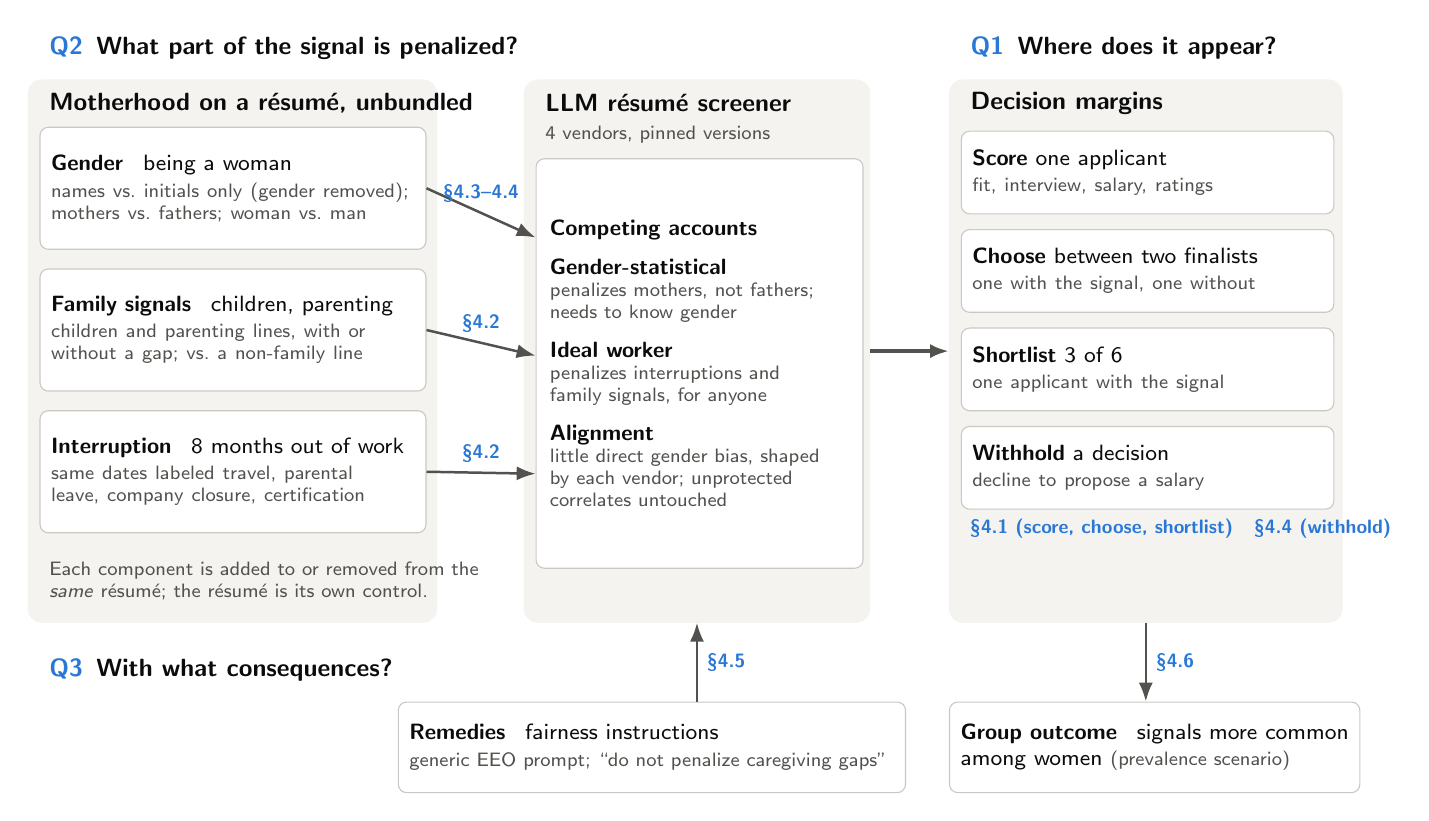
\begin{tikzpicture}[
  font=\footnotesize, color=ink,
  comp/.style={draw=rule, fill=white, rounded corners=3pt, text width=4.62cm, minimum height=1.55cm, align=left, inner sep=4pt, anchor=north west},
  marg/.style={draw=rule, fill=white, rounded corners=3pt, text width=4.45cm, minimum height=1.05cm, align=left, inner sep=4pt, anchor=north west},
  sect/.style={font=\scriptsize\bfseries, text=acc},
  q/.style={font=\small\bfseries, text=ink, anchor=west},
  note/.style={font=\scriptsize, text=ink2, align=left},
  arr/.style={-{Latex[length=2.4mm]}, line width=0.9pt, draw=ink2},
  big/.style={-{Latex[length=3mm]}, line width=2.6pt, draw=acc},
  thin/.style={-{Latex[length=2.2mm]}, line width=0.8pt, draw=ink2, dash pattern=on 2.5pt off 1.5pt},
]
% ---------------- column titles / questions
\node[q] at (0,7.55) {\textcolor{acc}{Q2}\enspace What part of the signal is penalized?};
\node[q] at (11.7,7.55) {\textcolor{acc}{Q1}\enspace Where does it appear?};

% ---------------- A: the unbundled signal
\begin{scope}[on background layer]
\fill[pane, rounded corners=5pt] (-0.15,7.15) rectangle (5.05,0.25);
\end{scope}
\node[font=\small\bfseries, anchor=west] at (0,6.85) {Motherhood on a r\'esum\'e, unbundled};
\node[comp] (G) at (0.0,6.55) {\textbf{Gender} \enspace being a woman\\[2pt]
  \parbox{4.6cm}{\raggedright\scriptsize\color{ink2}names vs.\ initials only (gender removed);\\ mothers vs.\ fathers; woman vs.\ man}};
\node[comp] (F) at (0.0,4.75) {\textbf{Family signals} \enspace children, parenting\\[2pt]
  \parbox{4.6cm}{\raggedright\scriptsize\color{ink2}children and parenting lines, with or\\ without a gap; vs.\ a non-family line}};
\node[comp] (I) at (0.0,2.95) {\textbf{Interruption} \enspace 8 months out of work\\[2pt]
  \parbox{4.6cm}{\raggedright\scriptsize\color{ink2}same dates labeled travel, parental\\ leave, company closure, certification}};
\node[note, anchor=north west] at (0,1.15) {Each component is added to or removed from the\\ \emph{same} r\'esum\'e; the r\'esum\'e is its own control.};

% ---------------- B: the screener
\begin{scope}[on background layer]
\fill[pane, rounded corners=5pt] (6.15,7.15) rectangle (10.55,0.25);
\end{scope}
\node[font=\small\bfseries, anchor=west] at (6.3,6.85) {LLM r\'esum\'e screener};
\node[note, anchor=west] at (6.3,6.45) {4 vendors, pinned versions};
\if\RESULTS0
  \node[draw=rule, fill=white, rounded corners=3pt, anchor=north west, minimum width=4.1cm, minimum height=5.2cm, align=left, inner sep=5pt] (S) at (6.3,6.15) {%
    \parbox{3.8cm}{\textbf{Competing accounts}\\[6pt]
    \textbf{Gender-statistical}\\ \scriptsize\color{ink2} penalizes mothers, not fathers;\\ needs to know gender\\[6pt]
    \normalsize\footnotesize\color{ink}\textbf{Ideal worker}\\ \scriptsize\color{ink2} penalizes interruptions and\\ family signals, for anyone\\[6pt]
    \normalsize\footnotesize\color{ink}\textbf{Alignment}\\ \scriptsize\color{ink2} little direct gender bias, shaped\\ by each vendor; unprotected\\ correlates untouched}};
  \draw[arr] (G.east) -- ($(S.west)+(0,1.6)$) node[midway, above, sect] {\S4.3--4.4};
  \draw[arr] (F.east) -- ($(S.west)+(0,0.1)$) node[midway, above, sect] {\S4.2};
  \draw[arr] (I.east) -- ($(S.west)+(0,-1.4)$) node[midway, above, sect] {\S4.2};
\else
  \node[draw=acc, fill=accl, rounded corners=3pt, anchor=north west, minimum width=4.1cm, minimum height=2.95cm, align=left, inner sep=5pt] (L1) at (6.3,6.15) {%
    \parbox{3.8cm}{\textbf{Layer 1: ideal-worker rule}\\[2pt]\scriptsize gender-blind; same for all vendors in sign\\[3pt]
    \textbullet\ interruption $\to$ availability\\ \phantom{\textbullet\ }inference (instruction reaches it)\\
    \textbullet\ family signals $\to$ norm\\ \phantom{\textbullet\ }(instruction does not)}};
  \node[draw=rule, fill=white, rounded corners=3pt, anchor=north west, minimum width=4.1cm, minimum height=1.9cm, align=left, inner sep=5pt] (L2) at (6.3,2.85) {%
    \parbox{3.8cm}{\textbf{Layer 2: gender layer}\\[2pt]\scriptsize thin; differs by vendor; surfaces\\ when gender is explicit\\ (pro-woman, anti-mother, parity)}};
  \draw[thin] (G.east) -- ($(L2.west)+(0,0.25)$) node[pos=0.18, right, font=\scriptsize, text=ink2] {weak};
  \draw[big] (F.east) -- ($(L1.west)+(0,0.25)$);
  \draw[big] (I.east) -- ($(L1.west)+(0,-0.9)$);
  \node[font=\scriptsize\bfseries, text=acc, anchor=west] at (5.08,2.35) {strong};
\fi

% ---------------- C: decision margins
\begin{scope}[on background layer]
\fill[pane, rounded corners=5pt] (11.55,7.15) rectangle (16.55,0.25);
\end{scope}
\node[font=\small\bfseries, anchor=west] at (11.7,6.85) {Decision margins};
\if\RESULTS0
  \node[marg] (M1) at (11.7,6.5) {\textbf{Score} one applicant\\ \scriptsize\color{ink2}fit, interview, salary, ratings};
  \node[marg] (M2) at (11.7,5.25) {\textbf{Choose} between two finalists\\ \scriptsize\color{ink2}one with the signal, one without};
  \node[marg] (M3) at (11.7,4.0) {\textbf{Shortlist} 3 of 6\\ \scriptsize\color{ink2}one applicant with the signal};
  \node[marg] (M4) at (11.7,2.75) {\textbf{Withhold} a decision\\ \scriptsize\color{ink2}decline to propose a salary};
  \node[sect, anchor=west] at (11.7,1.45) {\S4.1 (score, choose, shortlist)\quad \S4.4 (withhold)};
\else
  \node[marg] (M1) at (11.7,6.5) {\textbf{Score}: \enspace barely moves\\ \scriptsize\color{ink2}$\le$0.35 of 10 fit points};
  \node[marg, draw=acc, line width=0.9pt] (M2) at (11.7,5.25) {\textbf{Choose}: \enspace large penalty\\ \scriptsize\color{ink2}with leave: chosen 11--31\%, not 50\%};
  \node[marg, draw=acc, line width=0.9pt] (M3) at (11.7,4.0) {\textbf{Shortlist}: \enspace large penalty\\ \scriptsize\color{ink2}mothers: 25--78\% of childless rate};
  \node[marg] (M4) at (11.7,2.75) {\textbf{Withhold}: \enspace one vendor\\ \scriptsize\color{ink2}no salary: 20\% of pregnant applicants};
  \node[note, anchor=west] at (11.7,1.45) {Penalty is comparative: invisible to\\ single-applicant scoring audits.};
\fi
\draw[arr, line width=1.6pt] (10.55,3.7) -- (11.55,3.7);

% ---------------- D: consequences
\node[q] at (0,-0.35) {\textcolor{acc}{Q3}\enspace With what consequences?};
\node[draw=rule, fill=white, rounded corners=3pt, anchor=north west, minimum width=6.0cm, minimum height=1.15cm, align=left, inner sep=4pt] (R) at (4.55,-0.75) {%
  \if\RESULTS0 \textbf{Remedies} \enspace fairness instructions\\ \scriptsize\color{ink2}generic EEO prompt; ``do not penalize caregiving gaps''
  \else \textbf{Remedies}: \enspace reach interruption, not family\\ \scriptsize\color{ink2}generic prompt helps, does nothing, or backfires\fi};
\node[draw=rule, fill=white, rounded corners=3pt, anchor=north west, minimum width=5.0cm, minimum height=1.15cm, align=left, inner sep=4pt] (O) at (11.55,-0.75) {%
  \if\RESULTS0 \textbf{Group outcome} \enspace signals more common\\ among women \scriptsize\color{ink2}(prevalence scenario)
  \else \textbf{Group outcome}: \enspace gender-blind rule,\\ gendered result \scriptsize\color{ink2}(Haiku: four-fifths line at 31\%)\fi};
\draw[{Latex[length=2.4mm]}-, line width=0.9pt, draw=ink2] (8.35,0.25) -- (8.35,-0.75) node[pos=0.5, right, sect] {\S4.5};
\draw[arr] (14.05,0.25) -- (14.05,-0.75) node[pos=0.5, right, sect] {\S4.6};
\end{tikzpicture}
\end{document}
"  -> framework view
%          pdflatex "\def\RESULTS{1}% Figure 1 (framework) and Figure 9 (findings mapped onto the same framework).
% Compile: pdflatex "\def\RESULTS{0}% Figure 1 (framework) and Figure 9 (findings mapped onto the same framework).
% Compile: pdflatex "\def\RESULTS{0}\input{framework}"  -> framework view
%          pdflatex "\def\RESULTS{1}\input{framework}"  -> findings view
\documentclass[border=4pt]{standalone}
\usepackage[T1]{fontenc}
\usepackage{helvet}\renewcommand{\familydefault}{\sfdefault}
\usepackage{tikz}
\usetikzlibrary{positioning,arrows.meta,calc,fit,backgrounds}
\ifdefined\RESULTS\else\def\RESULTS{0}\fi
\definecolor{ink}{HTML}{0B0B0B}\definecolor{ink2}{HTML}{52514E}
\definecolor{acc}{HTML}{2A78D6}\definecolor{accl}{HTML}{E3EEFB}
\definecolor{pane}{HTML}{F4F3F0}\definecolor{rule}{HTML}{C9C8C2}
\begin{document}
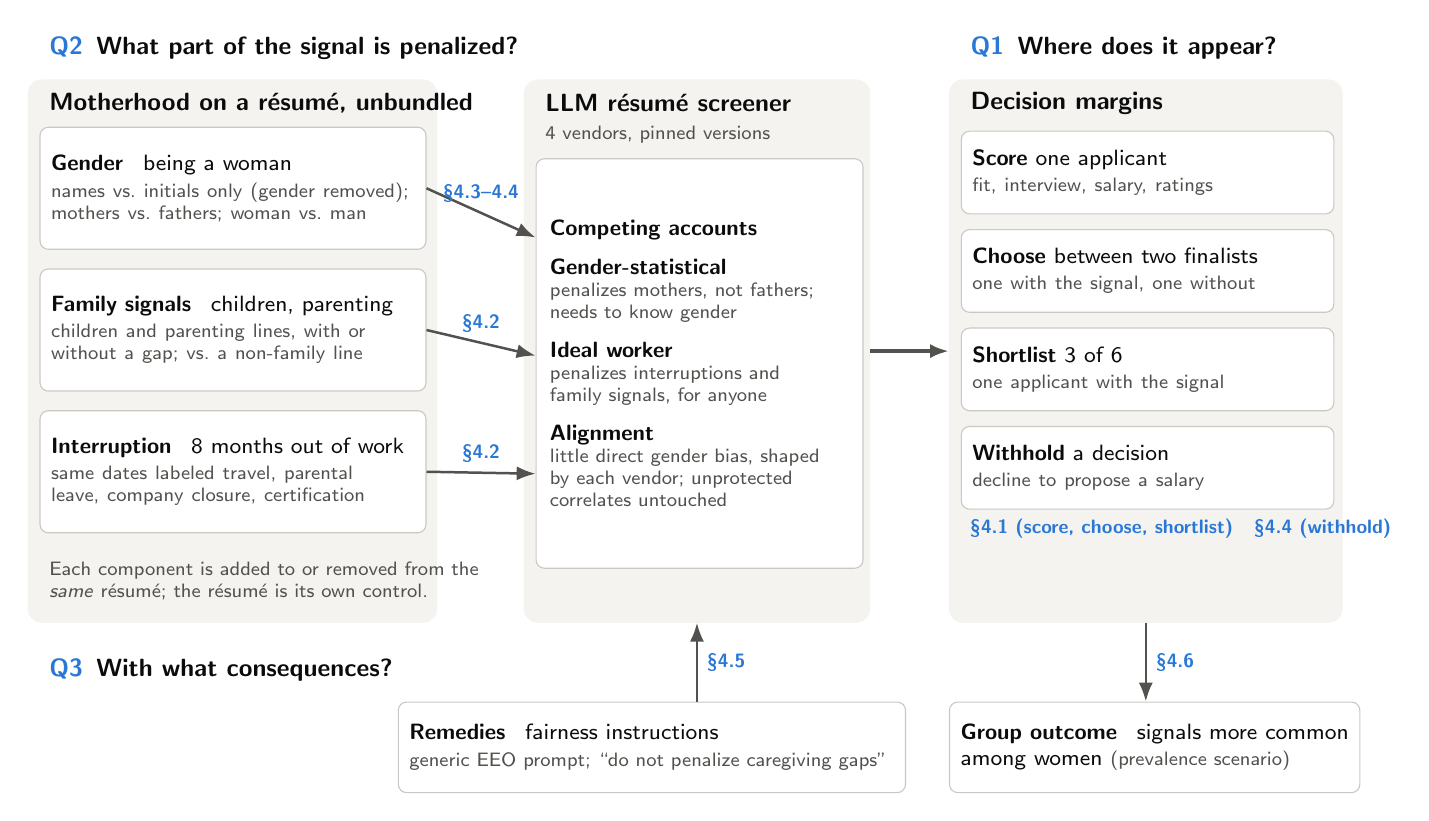
\begin{tikzpicture}[
  font=\footnotesize, color=ink,
  comp/.style={draw=rule, fill=white, rounded corners=3pt, text width=4.62cm, minimum height=1.55cm, align=left, inner sep=4pt, anchor=north west},
  marg/.style={draw=rule, fill=white, rounded corners=3pt, text width=4.45cm, minimum height=1.05cm, align=left, inner sep=4pt, anchor=north west},
  sect/.style={font=\scriptsize\bfseries, text=acc},
  q/.style={font=\small\bfseries, text=ink, anchor=west},
  note/.style={font=\scriptsize, text=ink2, align=left},
  arr/.style={-{Latex[length=2.4mm]}, line width=0.9pt, draw=ink2},
  big/.style={-{Latex[length=3mm]}, line width=2.6pt, draw=acc},
  thin/.style={-{Latex[length=2.2mm]}, line width=0.8pt, draw=ink2, dash pattern=on 2.5pt off 1.5pt},
]
% ---------------- column titles / questions
\node[q] at (0,7.55) {\textcolor{acc}{Q2}\enspace What part of the signal is penalized?};
\node[q] at (11.7,7.55) {\textcolor{acc}{Q1}\enspace Where does it appear?};

% ---------------- A: the unbundled signal
\begin{scope}[on background layer]
\fill[pane, rounded corners=5pt] (-0.15,7.15) rectangle (5.05,0.25);
\end{scope}
\node[font=\small\bfseries, anchor=west] at (0,6.85) {Motherhood on a r\'esum\'e, unbundled};
\node[comp] (G) at (0.0,6.55) {\textbf{Gender} \enspace being a woman\\[2pt]
  \parbox{4.6cm}{\raggedright\scriptsize\color{ink2}names vs.\ initials only (gender removed);\\ mothers vs.\ fathers; woman vs.\ man}};
\node[comp] (F) at (0.0,4.75) {\textbf{Family signals} \enspace children, parenting\\[2pt]
  \parbox{4.6cm}{\raggedright\scriptsize\color{ink2}children and parenting lines, with or\\ without a gap; vs.\ a non-family line}};
\node[comp] (I) at (0.0,2.95) {\textbf{Interruption} \enspace 8 months out of work\\[2pt]
  \parbox{4.6cm}{\raggedright\scriptsize\color{ink2}same dates labeled travel, parental\\ leave, company closure, certification}};
\node[note, anchor=north west] at (0,1.15) {Each component is added to or removed from the\\ \emph{same} r\'esum\'e; the r\'esum\'e is its own control.};

% ---------------- B: the screener
\begin{scope}[on background layer]
\fill[pane, rounded corners=5pt] (6.15,7.15) rectangle (10.55,0.25);
\end{scope}
\node[font=\small\bfseries, anchor=west] at (6.3,6.85) {LLM r\'esum\'e screener};
\node[note, anchor=west] at (6.3,6.45) {4 vendors, pinned versions};
\if\RESULTS0
  \node[draw=rule, fill=white, rounded corners=3pt, anchor=north west, minimum width=4.1cm, minimum height=5.2cm, align=left, inner sep=5pt] (S) at (6.3,6.15) {%
    \parbox{3.8cm}{\textbf{Competing accounts}\\[6pt]
    \textbf{Gender-statistical}\\ \scriptsize\color{ink2} penalizes mothers, not fathers;\\ needs to know gender\\[6pt]
    \normalsize\footnotesize\color{ink}\textbf{Ideal worker}\\ \scriptsize\color{ink2} penalizes interruptions and\\ family signals, for anyone\\[6pt]
    \normalsize\footnotesize\color{ink}\textbf{Alignment}\\ \scriptsize\color{ink2} little direct gender bias, shaped\\ by each vendor; unprotected\\ correlates untouched}};
  \draw[arr] (G.east) -- ($(S.west)+(0,1.6)$) node[midway, above, sect] {\S4.3--4.4};
  \draw[arr] (F.east) -- ($(S.west)+(0,0.1)$) node[midway, above, sect] {\S4.2};
  \draw[arr] (I.east) -- ($(S.west)+(0,-1.4)$) node[midway, above, sect] {\S4.2};
\else
  \node[draw=acc, fill=accl, rounded corners=3pt, anchor=north west, minimum width=4.1cm, minimum height=2.95cm, align=left, inner sep=5pt] (L1) at (6.3,6.15) {%
    \parbox{3.8cm}{\textbf{Layer 1: ideal-worker rule}\\[2pt]\scriptsize gender-blind; same for all vendors in sign\\[3pt]
    \textbullet\ interruption $\to$ availability\\ \phantom{\textbullet\ }inference (instruction reaches it)\\
    \textbullet\ family signals $\to$ norm\\ \phantom{\textbullet\ }(instruction does not)}};
  \node[draw=rule, fill=white, rounded corners=3pt, anchor=north west, minimum width=4.1cm, minimum height=1.9cm, align=left, inner sep=5pt] (L2) at (6.3,2.85) {%
    \parbox{3.8cm}{\textbf{Layer 2: gender layer}\\[2pt]\scriptsize thin; differs by vendor; surfaces\\ when gender is explicit\\ (pro-woman, anti-mother, parity)}};
  \draw[thin] (G.east) -- ($(L2.west)+(0,0.25)$) node[pos=0.18, right, font=\scriptsize, text=ink2] {weak};
  \draw[big] (F.east) -- ($(L1.west)+(0,0.25)$);
  \draw[big] (I.east) -- ($(L1.west)+(0,-0.9)$);
  \node[font=\scriptsize\bfseries, text=acc, anchor=west] at (5.08,2.35) {strong};
\fi

% ---------------- C: decision margins
\begin{scope}[on background layer]
\fill[pane, rounded corners=5pt] (11.55,7.15) rectangle (16.55,0.25);
\end{scope}
\node[font=\small\bfseries, anchor=west] at (11.7,6.85) {Decision margins};
\if\RESULTS0
  \node[marg] (M1) at (11.7,6.5) {\textbf{Score} one applicant\\ \scriptsize\color{ink2}fit, interview, salary, ratings};
  \node[marg] (M2) at (11.7,5.25) {\textbf{Choose} between two finalists\\ \scriptsize\color{ink2}one with the signal, one without};
  \node[marg] (M3) at (11.7,4.0) {\textbf{Shortlist} 3 of 6\\ \scriptsize\color{ink2}one applicant with the signal};
  \node[marg] (M4) at (11.7,2.75) {\textbf{Withhold} a decision\\ \scriptsize\color{ink2}decline to propose a salary};
  \node[sect, anchor=west] at (11.7,1.45) {\S4.1 (score, choose, shortlist)\quad \S4.4 (withhold)};
\else
  \node[marg] (M1) at (11.7,6.5) {\textbf{Score}: \enspace barely moves\\ \scriptsize\color{ink2}$\le$0.35 of 10 fit points};
  \node[marg, draw=acc, line width=0.9pt] (M2) at (11.7,5.25) {\textbf{Choose}: \enspace large penalty\\ \scriptsize\color{ink2}with leave: chosen 11--31\%, not 50\%};
  \node[marg, draw=acc, line width=0.9pt] (M3) at (11.7,4.0) {\textbf{Shortlist}: \enspace large penalty\\ \scriptsize\color{ink2}mothers: 25--78\% of childless rate};
  \node[marg] (M4) at (11.7,2.75) {\textbf{Withhold}: \enspace one vendor\\ \scriptsize\color{ink2}no salary: 20\% of pregnant applicants};
  \node[note, anchor=west] at (11.7,1.45) {Penalty is comparative: invisible to\\ single-applicant scoring audits.};
\fi
\draw[arr, line width=1.6pt] (10.55,3.7) -- (11.55,3.7);

% ---------------- D: consequences
\node[q] at (0,-0.35) {\textcolor{acc}{Q3}\enspace With what consequences?};
\node[draw=rule, fill=white, rounded corners=3pt, anchor=north west, minimum width=6.0cm, minimum height=1.15cm, align=left, inner sep=4pt] (R) at (4.55,-0.75) {%
  \if\RESULTS0 \textbf{Remedies} \enspace fairness instructions\\ \scriptsize\color{ink2}generic EEO prompt; ``do not penalize caregiving gaps''
  \else \textbf{Remedies}: \enspace reach interruption, not family\\ \scriptsize\color{ink2}generic prompt helps, does nothing, or backfires\fi};
\node[draw=rule, fill=white, rounded corners=3pt, anchor=north west, minimum width=5.0cm, minimum height=1.15cm, align=left, inner sep=4pt] (O) at (11.55,-0.75) {%
  \if\RESULTS0 \textbf{Group outcome} \enspace signals more common\\ among women \scriptsize\color{ink2}(prevalence scenario)
  \else \textbf{Group outcome}: \enspace gender-blind rule,\\ gendered result \scriptsize\color{ink2}(Haiku: four-fifths line at 31\%)\fi};
\draw[{Latex[length=2.4mm]}-, line width=0.9pt, draw=ink2] (8.35,0.25) -- (8.35,-0.75) node[pos=0.5, right, sect] {\S4.5};
\draw[arr] (14.05,0.25) -- (14.05,-0.75) node[pos=0.5, right, sect] {\S4.6};
\end{tikzpicture}
\end{document}
"  -> framework view
%          pdflatex "\def\RESULTS{1}% Figure 1 (framework) and Figure 9 (findings mapped onto the same framework).
% Compile: pdflatex "\def\RESULTS{0}\input{framework}"  -> framework view
%          pdflatex "\def\RESULTS{1}\input{framework}"  -> findings view
\documentclass[border=4pt]{standalone}
\usepackage[T1]{fontenc}
\usepackage{helvet}\renewcommand{\familydefault}{\sfdefault}
\usepackage{tikz}
\usetikzlibrary{positioning,arrows.meta,calc,fit,backgrounds}
\ifdefined\RESULTS\else\def\RESULTS{0}\fi
\definecolor{ink}{HTML}{0B0B0B}\definecolor{ink2}{HTML}{52514E}
\definecolor{acc}{HTML}{2A78D6}\definecolor{accl}{HTML}{E3EEFB}
\definecolor{pane}{HTML}{F4F3F0}\definecolor{rule}{HTML}{C9C8C2}
\begin{document}
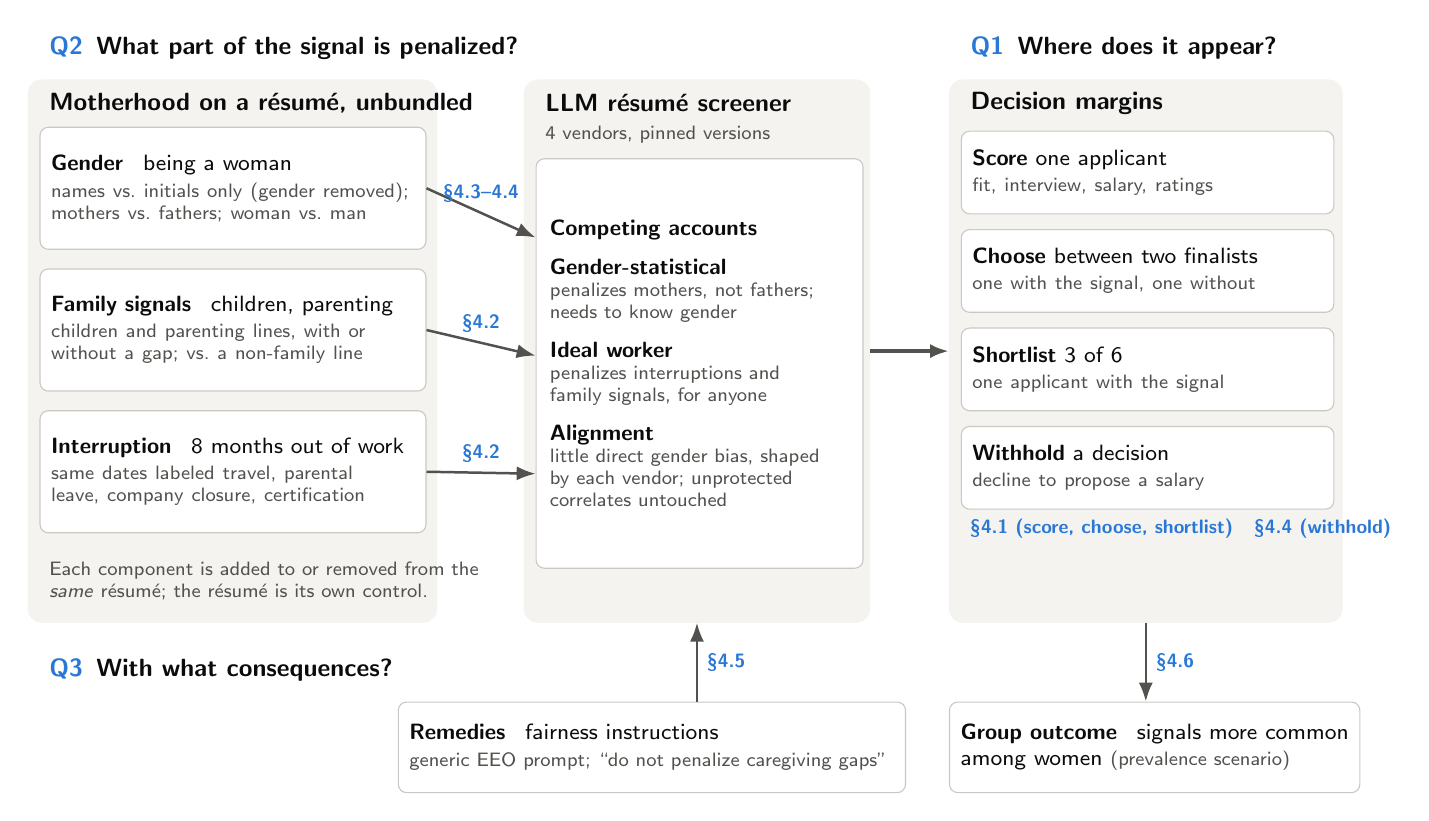
\begin{tikzpicture}[
  font=\footnotesize, color=ink,
  comp/.style={draw=rule, fill=white, rounded corners=3pt, text width=4.62cm, minimum height=1.55cm, align=left, inner sep=4pt, anchor=north west},
  marg/.style={draw=rule, fill=white, rounded corners=3pt, text width=4.45cm, minimum height=1.05cm, align=left, inner sep=4pt, anchor=north west},
  sect/.style={font=\scriptsize\bfseries, text=acc},
  q/.style={font=\small\bfseries, text=ink, anchor=west},
  note/.style={font=\scriptsize, text=ink2, align=left},
  arr/.style={-{Latex[length=2.4mm]}, line width=0.9pt, draw=ink2},
  big/.style={-{Latex[length=3mm]}, line width=2.6pt, draw=acc},
  thin/.style={-{Latex[length=2.2mm]}, line width=0.8pt, draw=ink2, dash pattern=on 2.5pt off 1.5pt},
]
% ---------------- column titles / questions
\node[q] at (0,7.55) {\textcolor{acc}{Q2}\enspace What part of the signal is penalized?};
\node[q] at (11.7,7.55) {\textcolor{acc}{Q1}\enspace Where does it appear?};

% ---------------- A: the unbundled signal
\begin{scope}[on background layer]
\fill[pane, rounded corners=5pt] (-0.15,7.15) rectangle (5.05,0.25);
\end{scope}
\node[font=\small\bfseries, anchor=west] at (0,6.85) {Motherhood on a r\'esum\'e, unbundled};
\node[comp] (G) at (0.0,6.55) {\textbf{Gender} \enspace being a woman\\[2pt]
  \parbox{4.6cm}{\raggedright\scriptsize\color{ink2}names vs.\ initials only (gender removed);\\ mothers vs.\ fathers; woman vs.\ man}};
\node[comp] (F) at (0.0,4.75) {\textbf{Family signals} \enspace children, parenting\\[2pt]
  \parbox{4.6cm}{\raggedright\scriptsize\color{ink2}children and parenting lines, with or\\ without a gap; vs.\ a non-family line}};
\node[comp] (I) at (0.0,2.95) {\textbf{Interruption} \enspace 8 months out of work\\[2pt]
  \parbox{4.6cm}{\raggedright\scriptsize\color{ink2}same dates labeled travel, parental\\ leave, company closure, certification}};
\node[note, anchor=north west] at (0,1.15) {Each component is added to or removed from the\\ \emph{same} r\'esum\'e; the r\'esum\'e is its own control.};

% ---------------- B: the screener
\begin{scope}[on background layer]
\fill[pane, rounded corners=5pt] (6.15,7.15) rectangle (10.55,0.25);
\end{scope}
\node[font=\small\bfseries, anchor=west] at (6.3,6.85) {LLM r\'esum\'e screener};
\node[note, anchor=west] at (6.3,6.45) {4 vendors, pinned versions};
\if\RESULTS0
  \node[draw=rule, fill=white, rounded corners=3pt, anchor=north west, minimum width=4.1cm, minimum height=5.2cm, align=left, inner sep=5pt] (S) at (6.3,6.15) {%
    \parbox{3.8cm}{\textbf{Competing accounts}\\[6pt]
    \textbf{Gender-statistical}\\ \scriptsize\color{ink2} penalizes mothers, not fathers;\\ needs to know gender\\[6pt]
    \normalsize\footnotesize\color{ink}\textbf{Ideal worker}\\ \scriptsize\color{ink2} penalizes interruptions and\\ family signals, for anyone\\[6pt]
    \normalsize\footnotesize\color{ink}\textbf{Alignment}\\ \scriptsize\color{ink2} little direct gender bias, shaped\\ by each vendor; unprotected\\ correlates untouched}};
  \draw[arr] (G.east) -- ($(S.west)+(0,1.6)$) node[midway, above, sect] {\S4.3--4.4};
  \draw[arr] (F.east) -- ($(S.west)+(0,0.1)$) node[midway, above, sect] {\S4.2};
  \draw[arr] (I.east) -- ($(S.west)+(0,-1.4)$) node[midway, above, sect] {\S4.2};
\else
  \node[draw=acc, fill=accl, rounded corners=3pt, anchor=north west, minimum width=4.1cm, minimum height=2.95cm, align=left, inner sep=5pt] (L1) at (6.3,6.15) {%
    \parbox{3.8cm}{\textbf{Layer 1: ideal-worker rule}\\[2pt]\scriptsize gender-blind; same for all vendors in sign\\[3pt]
    \textbullet\ interruption $\to$ availability\\ \phantom{\textbullet\ }inference (instruction reaches it)\\
    \textbullet\ family signals $\to$ norm\\ \phantom{\textbullet\ }(instruction does not)}};
  \node[draw=rule, fill=white, rounded corners=3pt, anchor=north west, minimum width=4.1cm, minimum height=1.9cm, align=left, inner sep=5pt] (L2) at (6.3,2.85) {%
    \parbox{3.8cm}{\textbf{Layer 2: gender layer}\\[2pt]\scriptsize thin; differs by vendor; surfaces\\ when gender is explicit\\ (pro-woman, anti-mother, parity)}};
  \draw[thin] (G.east) -- ($(L2.west)+(0,0.25)$) node[pos=0.18, right, font=\scriptsize, text=ink2] {weak};
  \draw[big] (F.east) -- ($(L1.west)+(0,0.25)$);
  \draw[big] (I.east) -- ($(L1.west)+(0,-0.9)$);
  \node[font=\scriptsize\bfseries, text=acc, anchor=west] at (5.08,2.35) {strong};
\fi

% ---------------- C: decision margins
\begin{scope}[on background layer]
\fill[pane, rounded corners=5pt] (11.55,7.15) rectangle (16.55,0.25);
\end{scope}
\node[font=\small\bfseries, anchor=west] at (11.7,6.85) {Decision margins};
\if\RESULTS0
  \node[marg] (M1) at (11.7,6.5) {\textbf{Score} one applicant\\ \scriptsize\color{ink2}fit, interview, salary, ratings};
  \node[marg] (M2) at (11.7,5.25) {\textbf{Choose} between two finalists\\ \scriptsize\color{ink2}one with the signal, one without};
  \node[marg] (M3) at (11.7,4.0) {\textbf{Shortlist} 3 of 6\\ \scriptsize\color{ink2}one applicant with the signal};
  \node[marg] (M4) at (11.7,2.75) {\textbf{Withhold} a decision\\ \scriptsize\color{ink2}decline to propose a salary};
  \node[sect, anchor=west] at (11.7,1.45) {\S4.1 (score, choose, shortlist)\quad \S4.4 (withhold)};
\else
  \node[marg] (M1) at (11.7,6.5) {\textbf{Score}: \enspace barely moves\\ \scriptsize\color{ink2}$\le$0.35 of 10 fit points};
  \node[marg, draw=acc, line width=0.9pt] (M2) at (11.7,5.25) {\textbf{Choose}: \enspace large penalty\\ \scriptsize\color{ink2}with leave: chosen 11--31\%, not 50\%};
  \node[marg, draw=acc, line width=0.9pt] (M3) at (11.7,4.0) {\textbf{Shortlist}: \enspace large penalty\\ \scriptsize\color{ink2}mothers: 25--78\% of childless rate};
  \node[marg] (M4) at (11.7,2.75) {\textbf{Withhold}: \enspace one vendor\\ \scriptsize\color{ink2}no salary: 20\% of pregnant applicants};
  \node[note, anchor=west] at (11.7,1.45) {Penalty is comparative: invisible to\\ single-applicant scoring audits.};
\fi
\draw[arr, line width=1.6pt] (10.55,3.7) -- (11.55,3.7);

% ---------------- D: consequences
\node[q] at (0,-0.35) {\textcolor{acc}{Q3}\enspace With what consequences?};
\node[draw=rule, fill=white, rounded corners=3pt, anchor=north west, minimum width=6.0cm, minimum height=1.15cm, align=left, inner sep=4pt] (R) at (4.55,-0.75) {%
  \if\RESULTS0 \textbf{Remedies} \enspace fairness instructions\\ \scriptsize\color{ink2}generic EEO prompt; ``do not penalize caregiving gaps''
  \else \textbf{Remedies}: \enspace reach interruption, not family\\ \scriptsize\color{ink2}generic prompt helps, does nothing, or backfires\fi};
\node[draw=rule, fill=white, rounded corners=3pt, anchor=north west, minimum width=5.0cm, minimum height=1.15cm, align=left, inner sep=4pt] (O) at (11.55,-0.75) {%
  \if\RESULTS0 \textbf{Group outcome} \enspace signals more common\\ among women \scriptsize\color{ink2}(prevalence scenario)
  \else \textbf{Group outcome}: \enspace gender-blind rule,\\ gendered result \scriptsize\color{ink2}(Haiku: four-fifths line at 31\%)\fi};
\draw[{Latex[length=2.4mm]}-, line width=0.9pt, draw=ink2] (8.35,0.25) -- (8.35,-0.75) node[pos=0.5, right, sect] {\S4.5};
\draw[arr] (14.05,0.25) -- (14.05,-0.75) node[pos=0.5, right, sect] {\S4.6};
\end{tikzpicture}
\end{document}
"  -> findings view
\documentclass[border=4pt]{standalone}
\usepackage[T1]{fontenc}
\usepackage{helvet}\renewcommand{\familydefault}{\sfdefault}
\usepackage{tikz}
\usetikzlibrary{positioning,arrows.meta,calc,fit,backgrounds}
\ifdefined\RESULTS\else\def\RESULTS{0}\fi
\definecolor{ink}{HTML}{0B0B0B}\definecolor{ink2}{HTML}{52514E}
\definecolor{acc}{HTML}{2A78D6}\definecolor{accl}{HTML}{E3EEFB}
\definecolor{pane}{HTML}{F4F3F0}\definecolor{rule}{HTML}{C9C8C2}
\begin{document}
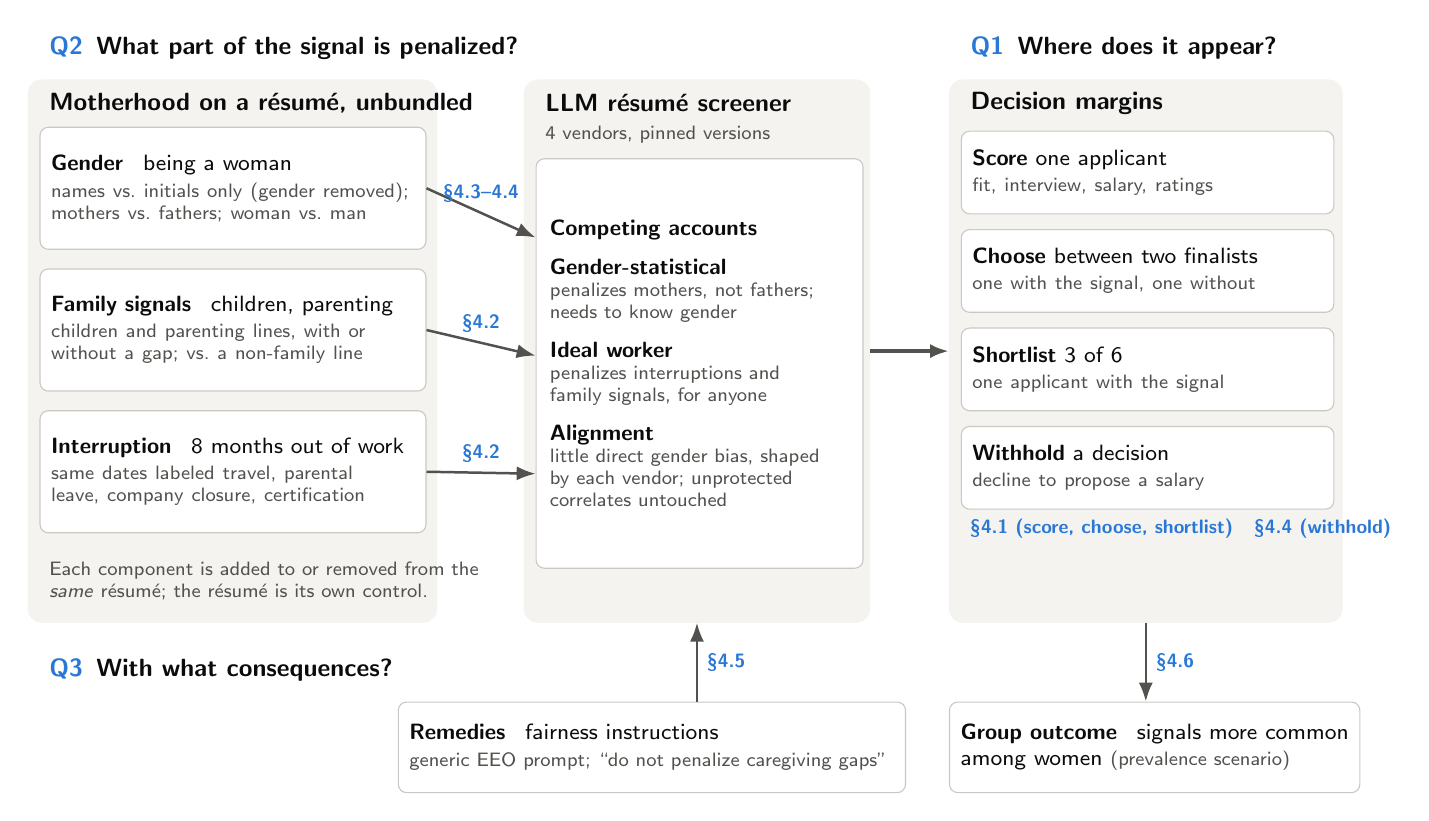
\begin{tikzpicture}[
  font=\footnotesize, color=ink,
  comp/.style={draw=rule, fill=white, rounded corners=3pt, text width=4.62cm, minimum height=1.55cm, align=left, inner sep=4pt, anchor=north west},
  marg/.style={draw=rule, fill=white, rounded corners=3pt, text width=4.45cm, minimum height=1.05cm, align=left, inner sep=4pt, anchor=north west},
  sect/.style={font=\scriptsize\bfseries, text=acc},
  q/.style={font=\small\bfseries, text=ink, anchor=west},
  note/.style={font=\scriptsize, text=ink2, align=left},
  arr/.style={-{Latex[length=2.4mm]}, line width=0.9pt, draw=ink2},
  big/.style={-{Latex[length=3mm]}, line width=2.6pt, draw=acc},
  thin/.style={-{Latex[length=2.2mm]}, line width=0.8pt, draw=ink2, dash pattern=on 2.5pt off 1.5pt},
]
% ---------------- column titles / questions
\node[q] at (0,7.55) {\textcolor{acc}{Q2}\enspace What part of the signal is penalized?};
\node[q] at (11.7,7.55) {\textcolor{acc}{Q1}\enspace Where does it appear?};

% ---------------- A: the unbundled signal
\begin{scope}[on background layer]
\fill[pane, rounded corners=5pt] (-0.15,7.15) rectangle (5.05,0.25);
\end{scope}
\node[font=\small\bfseries, anchor=west] at (0,6.85) {Motherhood on a r\'esum\'e, unbundled};
\node[comp] (G) at (0.0,6.55) {\textbf{Gender} \enspace being a woman\\[2pt]
  \parbox{4.6cm}{\raggedright\scriptsize\color{ink2}names vs.\ initials only (gender removed);\\ mothers vs.\ fathers; woman vs.\ man}};
\node[comp] (F) at (0.0,4.75) {\textbf{Family signals} \enspace children, parenting\\[2pt]
  \parbox{4.6cm}{\raggedright\scriptsize\color{ink2}children and parenting lines, with or\\ without a gap; vs.\ a non-family line}};
\node[comp] (I) at (0.0,2.95) {\textbf{Interruption} \enspace 8 months out of work\\[2pt]
  \parbox{4.6cm}{\raggedright\scriptsize\color{ink2}same dates labeled travel, parental\\ leave, company closure, certification}};
\node[note, anchor=north west] at (0,1.15) {Each component is added to or removed from the\\ \emph{same} r\'esum\'e; the r\'esum\'e is its own control.};

% ---------------- B: the screener
\begin{scope}[on background layer]
\fill[pane, rounded corners=5pt] (6.15,7.15) rectangle (10.55,0.25);
\end{scope}
\node[font=\small\bfseries, anchor=west] at (6.3,6.85) {LLM r\'esum\'e screener};
\node[note, anchor=west] at (6.3,6.45) {4 vendors, pinned versions};
\if\RESULTS0
  \node[draw=rule, fill=white, rounded corners=3pt, anchor=north west, minimum width=4.1cm, minimum height=5.2cm, align=left, inner sep=5pt] (S) at (6.3,6.15) {%
    \parbox{3.8cm}{\textbf{Competing accounts}\\[6pt]
    \textbf{Gender-statistical}\\ \scriptsize\color{ink2} penalizes mothers, not fathers;\\ needs to know gender\\[6pt]
    \normalsize\footnotesize\color{ink}\textbf{Ideal worker}\\ \scriptsize\color{ink2} penalizes interruptions and\\ family signals, for anyone\\[6pt]
    \normalsize\footnotesize\color{ink}\textbf{Alignment}\\ \scriptsize\color{ink2} little direct gender bias, shaped\\ by each vendor; unprotected\\ correlates untouched}};
  \draw[arr] (G.east) -- ($(S.west)+(0,1.6)$) node[midway, above, sect] {\S4.3--4.4};
  \draw[arr] (F.east) -- ($(S.west)+(0,0.1)$) node[midway, above, sect] {\S4.2};
  \draw[arr] (I.east) -- ($(S.west)+(0,-1.4)$) node[midway, above, sect] {\S4.2};
\else
  \node[draw=acc, fill=accl, rounded corners=3pt, anchor=north west, minimum width=4.1cm, minimum height=2.95cm, align=left, inner sep=5pt] (L1) at (6.3,6.15) {%
    \parbox{3.8cm}{\textbf{Layer 1: ideal-worker rule}\\[2pt]\scriptsize gender-blind; same for all vendors in sign\\[3pt]
    \textbullet\ interruption $\to$ availability\\ \phantom{\textbullet\ }inference (instruction reaches it)\\
    \textbullet\ family signals $\to$ norm\\ \phantom{\textbullet\ }(instruction does not)}};
  \node[draw=rule, fill=white, rounded corners=3pt, anchor=north west, minimum width=4.1cm, minimum height=1.9cm, align=left, inner sep=5pt] (L2) at (6.3,2.85) {%
    \parbox{3.8cm}{\textbf{Layer 2: gender layer}\\[2pt]\scriptsize thin; differs by vendor; surfaces\\ when gender is explicit\\ (pro-woman, anti-mother, parity)}};
  \draw[thin] (G.east) -- ($(L2.west)+(0,0.25)$) node[pos=0.18, right, font=\scriptsize, text=ink2] {weak};
  \draw[big] (F.east) -- ($(L1.west)+(0,0.25)$);
  \draw[big] (I.east) -- ($(L1.west)+(0,-0.9)$);
  \node[font=\scriptsize\bfseries, text=acc, anchor=west] at (5.08,2.35) {strong};
\fi

% ---------------- C: decision margins
\begin{scope}[on background layer]
\fill[pane, rounded corners=5pt] (11.55,7.15) rectangle (16.55,0.25);
\end{scope}
\node[font=\small\bfseries, anchor=west] at (11.7,6.85) {Decision margins};
\if\RESULTS0
  \node[marg] (M1) at (11.7,6.5) {\textbf{Score} one applicant\\ \scriptsize\color{ink2}fit, interview, salary, ratings};
  \node[marg] (M2) at (11.7,5.25) {\textbf{Choose} between two finalists\\ \scriptsize\color{ink2}one with the signal, one without};
  \node[marg] (M3) at (11.7,4.0) {\textbf{Shortlist} 3 of 6\\ \scriptsize\color{ink2}one applicant with the signal};
  \node[marg] (M4) at (11.7,2.75) {\textbf{Withhold} a decision\\ \scriptsize\color{ink2}decline to propose a salary};
  \node[sect, anchor=west] at (11.7,1.45) {\S4.1 (score, choose, shortlist)\quad \S4.4 (withhold)};
\else
  \node[marg] (M1) at (11.7,6.5) {\textbf{Score}: \enspace barely moves\\ \scriptsize\color{ink2}$\le$0.35 of 10 fit points};
  \node[marg, draw=acc, line width=0.9pt] (M2) at (11.7,5.25) {\textbf{Choose}: \enspace large penalty\\ \scriptsize\color{ink2}with leave: chosen 11--31\%, not 50\%};
  \node[marg, draw=acc, line width=0.9pt] (M3) at (11.7,4.0) {\textbf{Shortlist}: \enspace large penalty\\ \scriptsize\color{ink2}mothers: 25--78\% of childless rate};
  \node[marg] (M4) at (11.7,2.75) {\textbf{Withhold}: \enspace one vendor\\ \scriptsize\color{ink2}no salary: 20\% of pregnant applicants};
  \node[note, anchor=west] at (11.7,1.45) {Penalty is comparative: invisible to\\ single-applicant scoring audits.};
\fi
\draw[arr, line width=1.6pt] (10.55,3.7) -- (11.55,3.7);

% ---------------- D: consequences
\node[q] at (0,-0.35) {\textcolor{acc}{Q3}\enspace With what consequences?};
\node[draw=rule, fill=white, rounded corners=3pt, anchor=north west, minimum width=6.0cm, minimum height=1.15cm, align=left, inner sep=4pt] (R) at (4.55,-0.75) {%
  \if\RESULTS0 \textbf{Remedies} \enspace fairness instructions\\ \scriptsize\color{ink2}generic EEO prompt; ``do not penalize caregiving gaps''
  \else \textbf{Remedies}: \enspace reach interruption, not family\\ \scriptsize\color{ink2}generic prompt helps, does nothing, or backfires\fi};
\node[draw=rule, fill=white, rounded corners=3pt, anchor=north west, minimum width=5.0cm, minimum height=1.15cm, align=left, inner sep=4pt] (O) at (11.55,-0.75) {%
  \if\RESULTS0 \textbf{Group outcome} \enspace signals more common\\ among women \scriptsize\color{ink2}(prevalence scenario)
  \else \textbf{Group outcome}: \enspace gender-blind rule,\\ gendered result \scriptsize\color{ink2}(Haiku: four-fifths line at 31\%)\fi};
\draw[{Latex[length=2.4mm]}-, line width=0.9pt, draw=ink2] (8.35,0.25) -- (8.35,-0.75) node[pos=0.5, right, sect] {\S4.5};
\draw[arr] (14.05,0.25) -- (14.05,-0.75) node[pos=0.5, right, sect] {\S4.6};
\end{tikzpicture}
\end{document}
"  -> findings view
\documentclass[border=4pt]{standalone}
\usepackage[T1]{fontenc}
\usepackage{helvet}\renewcommand{\familydefault}{\sfdefault}
\usepackage{tikz}
\usetikzlibrary{positioning,arrows.meta,calc,fit,backgrounds}
\ifdefined\RESULTS\else\def\RESULTS{0}\fi
\definecolor{ink}{HTML}{0B0B0B}\definecolor{ink2}{HTML}{52514E}
\definecolor{acc}{HTML}{2A78D6}\definecolor{accl}{HTML}{E3EEFB}
\definecolor{pane}{HTML}{F4F3F0}\definecolor{rule}{HTML}{C9C8C2}
\begin{document}
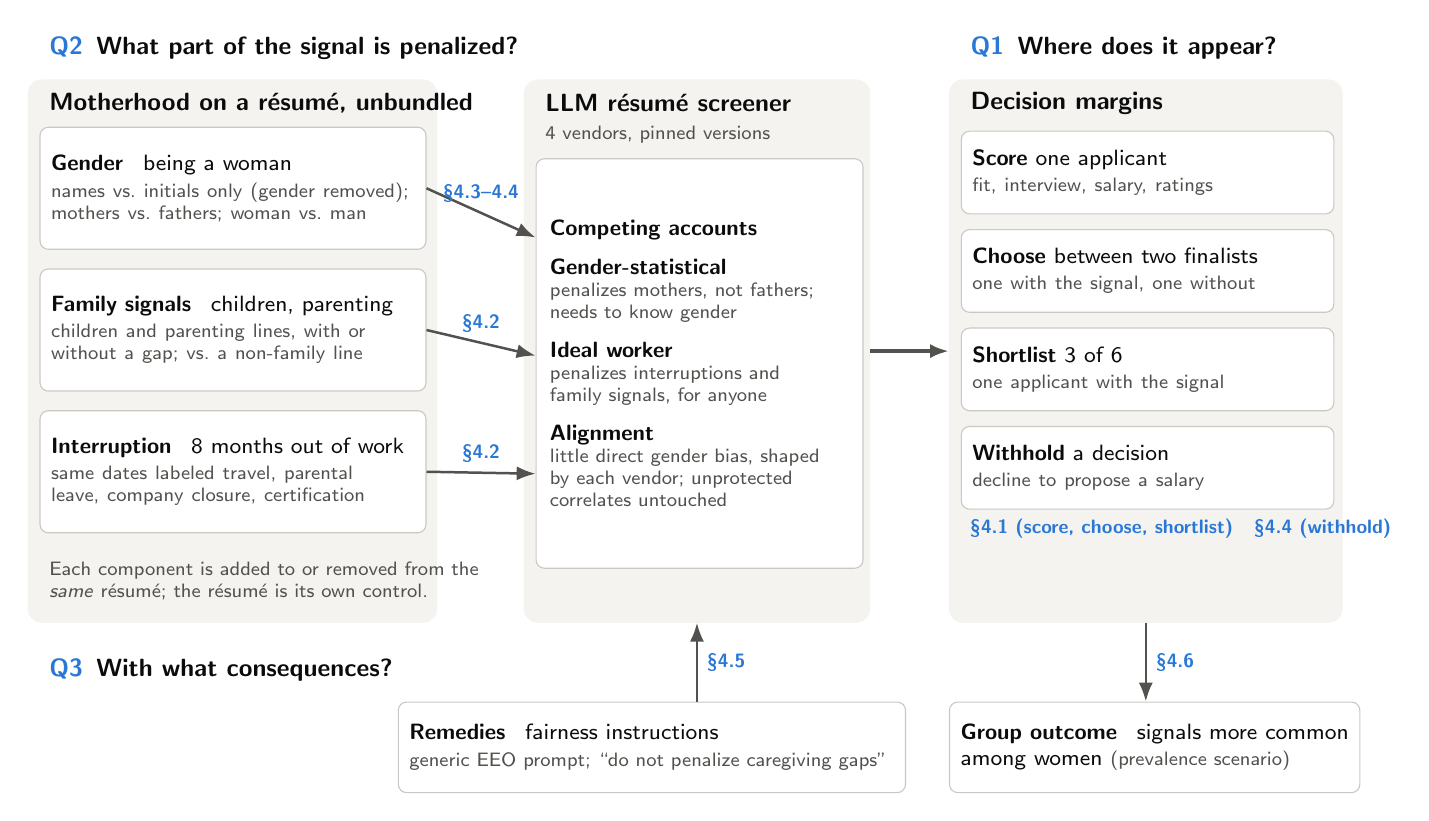
\begin{tikzpicture}[
  font=\footnotesize, color=ink,
  comp/.style={draw=rule, fill=white, rounded corners=3pt, text width=4.62cm, minimum height=1.55cm, align=left, inner sep=4pt, anchor=north west},
  marg/.style={draw=rule, fill=white, rounded corners=3pt, text width=4.45cm, minimum height=1.05cm, align=left, inner sep=4pt, anchor=north west},
  sect/.style={font=\scriptsize\bfseries, text=acc},
  q/.style={font=\small\bfseries, text=ink, anchor=west},
  note/.style={font=\scriptsize, text=ink2, align=left},
  arr/.style={-{Latex[length=2.4mm]}, line width=0.9pt, draw=ink2},
  big/.style={-{Latex[length=3mm]}, line width=2.6pt, draw=acc},
  thin/.style={-{Latex[length=2.2mm]}, line width=0.8pt, draw=ink2, dash pattern=on 2.5pt off 1.5pt},
]
% ---------------- column titles / questions
\node[q] at (0,7.55) {\textcolor{acc}{Q2}\enspace What part of the signal is penalized?};
\node[q] at (11.7,7.55) {\textcolor{acc}{Q1}\enspace Where does it appear?};

% ---------------- A: the unbundled signal
\begin{scope}[on background layer]
\fill[pane, rounded corners=5pt] (-0.15,7.15) rectangle (5.05,0.25);
\end{scope}
\node[font=\small\bfseries, anchor=west] at (0,6.85) {Motherhood on a r\'esum\'e, unbundled};
\node[comp] (G) at (0.0,6.55) {\textbf{Gender} \enspace being a woman\\[2pt]
  \parbox{4.6cm}{\raggedright\scriptsize\color{ink2}names vs.\ initials only (gender removed);\\ mothers vs.\ fathers; woman vs.\ man}};
\node[comp] (F) at (0.0,4.75) {\textbf{Family signals} \enspace children, parenting\\[2pt]
  \parbox{4.6cm}{\raggedright\scriptsize\color{ink2}children and parenting lines, with or\\ without a gap; vs.\ a non-family line}};
\node[comp] (I) at (0.0,2.95) {\textbf{Interruption} \enspace 8 months out of work\\[2pt]
  \parbox{4.6cm}{\raggedright\scriptsize\color{ink2}same dates labeled travel, parental\\ leave, company closure, certification}};
\node[note, anchor=north west] at (0,1.15) {Each component is added to or removed from the\\ \emph{same} r\'esum\'e; the r\'esum\'e is its own control.};

% ---------------- B: the screener
\begin{scope}[on background layer]
\fill[pane, rounded corners=5pt] (6.15,7.15) rectangle (10.55,0.25);
\end{scope}
\node[font=\small\bfseries, anchor=west] at (6.3,6.85) {LLM r\'esum\'e screener};
\node[note, anchor=west] at (6.3,6.45) {4 vendors, pinned versions};
\if\RESULTS0
  \node[draw=rule, fill=white, rounded corners=3pt, anchor=north west, minimum width=4.1cm, minimum height=5.2cm, align=left, inner sep=5pt] (S) at (6.3,6.15) {%
    \parbox{3.8cm}{\textbf{Competing accounts}\\[6pt]
    \textbf{Gender-statistical}\\ \scriptsize\color{ink2} penalizes mothers, not fathers;\\ needs to know gender\\[6pt]
    \normalsize\footnotesize\color{ink}\textbf{Ideal worker}\\ \scriptsize\color{ink2} penalizes interruptions and\\ family signals, for anyone\\[6pt]
    \normalsize\footnotesize\color{ink}\textbf{Alignment}\\ \scriptsize\color{ink2} little direct gender bias, shaped\\ by each vendor; unprotected\\ correlates untouched}};
  \draw[arr] (G.east) -- ($(S.west)+(0,1.6)$) node[midway, above, sect] {\S4.3--4.4};
  \draw[arr] (F.east) -- ($(S.west)+(0,0.1)$) node[midway, above, sect] {\S4.2};
  \draw[arr] (I.east) -- ($(S.west)+(0,-1.4)$) node[midway, above, sect] {\S4.2};
\else
  \node[draw=acc, fill=accl, rounded corners=3pt, anchor=north west, minimum width=4.1cm, minimum height=2.95cm, align=left, inner sep=5pt] (L1) at (6.3,6.15) {%
    \parbox{3.8cm}{\textbf{Layer 1: ideal-worker rule}\\[2pt]\scriptsize gender-blind; same for all vendors in sign\\[3pt]
    \textbullet\ interruption $\to$ availability\\ \phantom{\textbullet\ }inference (instruction reaches it)\\
    \textbullet\ family signals $\to$ norm\\ \phantom{\textbullet\ }(instruction does not)}};
  \node[draw=rule, fill=white, rounded corners=3pt, anchor=north west, minimum width=4.1cm, minimum height=1.9cm, align=left, inner sep=5pt] (L2) at (6.3,2.85) {%
    \parbox{3.8cm}{\textbf{Layer 2: gender layer}\\[2pt]\scriptsize thin; differs by vendor; surfaces\\ when gender is explicit\\ (pro-woman, anti-mother, parity)}};
  \draw[thin] (G.east) -- ($(L2.west)+(0,0.25)$) node[pos=0.18, right, font=\scriptsize, text=ink2] {weak};
  \draw[big] (F.east) -- ($(L1.west)+(0,0.25)$);
  \draw[big] (I.east) -- ($(L1.west)+(0,-0.9)$);
  \node[font=\scriptsize\bfseries, text=acc, anchor=west] at (5.08,2.35) {strong};
\fi

% ---------------- C: decision margins
\begin{scope}[on background layer]
\fill[pane, rounded corners=5pt] (11.55,7.15) rectangle (16.55,0.25);
\end{scope}
\node[font=\small\bfseries, anchor=west] at (11.7,6.85) {Decision margins};
\if\RESULTS0
  \node[marg] (M1) at (11.7,6.5) {\textbf{Score} one applicant\\ \scriptsize\color{ink2}fit, interview, salary, ratings};
  \node[marg] (M2) at (11.7,5.25) {\textbf{Choose} between two finalists\\ \scriptsize\color{ink2}one with the signal, one without};
  \node[marg] (M3) at (11.7,4.0) {\textbf{Shortlist} 3 of 6\\ \scriptsize\color{ink2}one applicant with the signal};
  \node[marg] (M4) at (11.7,2.75) {\textbf{Withhold} a decision\\ \scriptsize\color{ink2}decline to propose a salary};
  \node[sect, anchor=west] at (11.7,1.45) {\S4.1 (score, choose, shortlist)\quad \S4.4 (withhold)};
\else
  \node[marg] (M1) at (11.7,6.5) {\textbf{Score}: \enspace barely moves\\ \scriptsize\color{ink2}$\le$0.35 of 10 fit points};
  \node[marg, draw=acc, line width=0.9pt] (M2) at (11.7,5.25) {\textbf{Choose}: \enspace large penalty\\ \scriptsize\color{ink2}with leave: chosen 11--31\%, not 50\%};
  \node[marg, draw=acc, line width=0.9pt] (M3) at (11.7,4.0) {\textbf{Shortlist}: \enspace large penalty\\ \scriptsize\color{ink2}mothers: 25--78\% of childless rate};
  \node[marg] (M4) at (11.7,2.75) {\textbf{Withhold}: \enspace one vendor\\ \scriptsize\color{ink2}no salary: 20\% of pregnant applicants};
  \node[note, anchor=west] at (11.7,1.45) {Penalty is comparative: invisible to\\ single-applicant scoring audits.};
\fi
\draw[arr, line width=1.6pt] (10.55,3.7) -- (11.55,3.7);

% ---------------- D: consequences
\node[q] at (0,-0.35) {\textcolor{acc}{Q3}\enspace With what consequences?};
\node[draw=rule, fill=white, rounded corners=3pt, anchor=north west, minimum width=6.0cm, minimum height=1.15cm, align=left, inner sep=4pt] (R) at (4.55,-0.75) {%
  \if\RESULTS0 \textbf{Remedies} \enspace fairness instructions\\ \scriptsize\color{ink2}generic EEO prompt; ``do not penalize caregiving gaps''
  \else \textbf{Remedies}: \enspace reach interruption, not family\\ \scriptsize\color{ink2}generic prompt helps, does nothing, or backfires\fi};
\node[draw=rule, fill=white, rounded corners=3pt, anchor=north west, minimum width=5.0cm, minimum height=1.15cm, align=left, inner sep=4pt] (O) at (11.55,-0.75) {%
  \if\RESULTS0 \textbf{Group outcome} \enspace signals more common\\ among women \scriptsize\color{ink2}(prevalence scenario)
  \else \textbf{Group outcome}: \enspace gender-blind rule,\\ gendered result \scriptsize\color{ink2}(Haiku: four-fifths line at 31\%)\fi};
\draw[{Latex[length=2.4mm]}-, line width=0.9pt, draw=ink2] (8.35,0.25) -- (8.35,-0.75) node[pos=0.5, right, sect] {\S4.5};
\draw[arr] (14.05,0.25) -- (14.05,-0.75) node[pos=0.5, right, sect] {\S4.6};
\end{tikzpicture}
\end{document}
"  -> framework view
%          pdflatex "\def\RESULTS{1}% Figure 1 (framework) and Figure 9 (findings mapped onto the same framework).
% Compile: pdflatex "\def\RESULTS{0}% Figure 1 (framework) and Figure 9 (findings mapped onto the same framework).
% Compile: pdflatex "\def\RESULTS{0}% Figure 1 (framework) and Figure 9 (findings mapped onto the same framework).
% Compile: pdflatex "\def\RESULTS{0}\input{framework}"  -> framework view
%          pdflatex "\def\RESULTS{1}\input{framework}"  -> findings view
\documentclass[border=4pt]{standalone}
\usepackage[T1]{fontenc}
\usepackage{helvet}\renewcommand{\familydefault}{\sfdefault}
\usepackage{tikz}
\usetikzlibrary{positioning,arrows.meta,calc,fit,backgrounds}
\ifdefined\RESULTS\else\def\RESULTS{0}\fi
\definecolor{ink}{HTML}{0B0B0B}\definecolor{ink2}{HTML}{52514E}
\definecolor{acc}{HTML}{2A78D6}\definecolor{accl}{HTML}{E3EEFB}
\definecolor{pane}{HTML}{F4F3F0}\definecolor{rule}{HTML}{C9C8C2}
\begin{document}
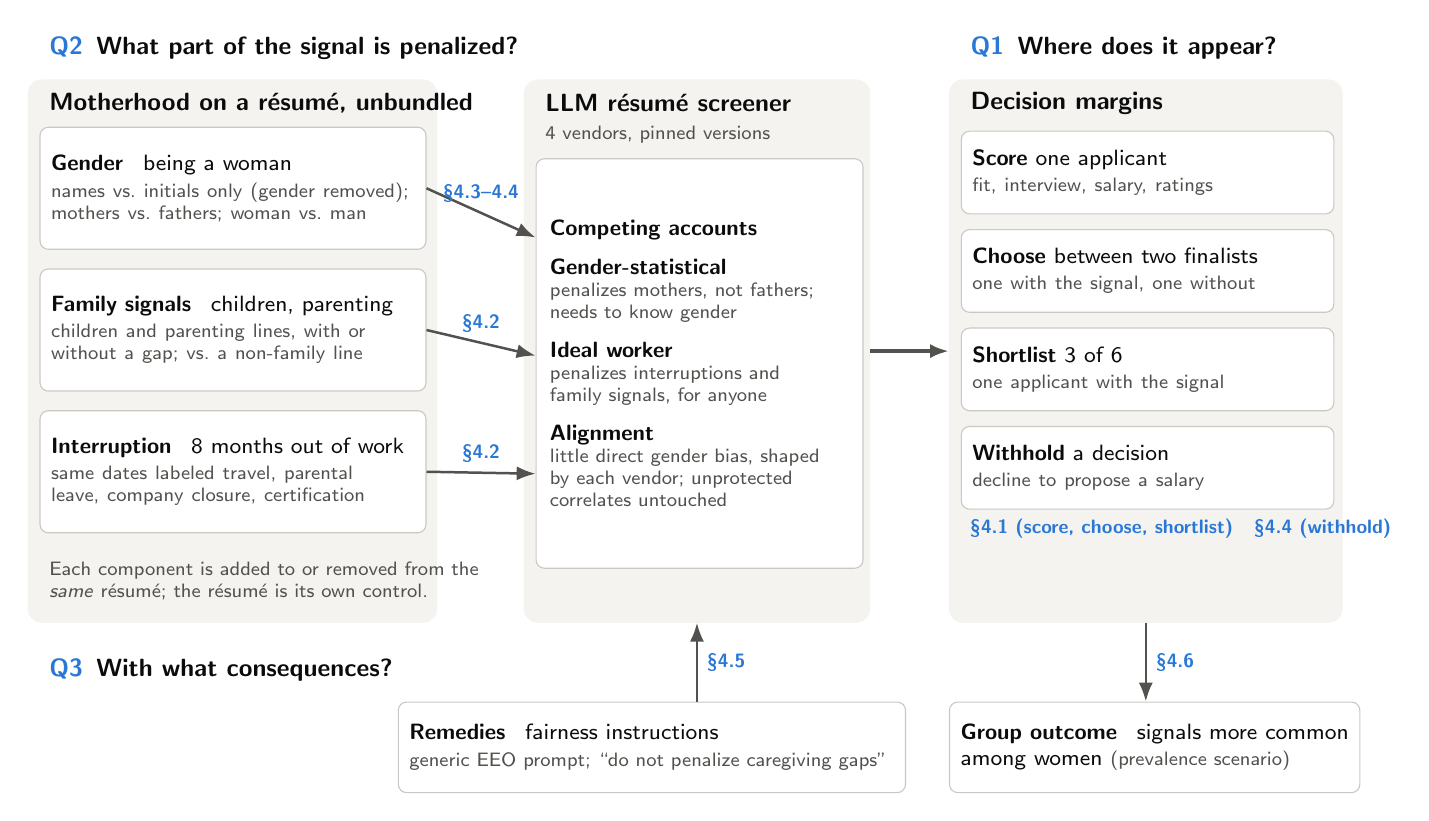
\begin{tikzpicture}[
  font=\footnotesize, color=ink,
  comp/.style={draw=rule, fill=white, rounded corners=3pt, text width=4.62cm, minimum height=1.55cm, align=left, inner sep=4pt, anchor=north west},
  marg/.style={draw=rule, fill=white, rounded corners=3pt, text width=4.45cm, minimum height=1.05cm, align=left, inner sep=4pt, anchor=north west},
  sect/.style={font=\scriptsize\bfseries, text=acc},
  q/.style={font=\small\bfseries, text=ink, anchor=west},
  note/.style={font=\scriptsize, text=ink2, align=left},
  arr/.style={-{Latex[length=2.4mm]}, line width=0.9pt, draw=ink2},
  big/.style={-{Latex[length=3mm]}, line width=2.6pt, draw=acc},
  thin/.style={-{Latex[length=2.2mm]}, line width=0.8pt, draw=ink2, dash pattern=on 2.5pt off 1.5pt},
]
% ---------------- column titles / questions
\node[q] at (0,7.55) {\textcolor{acc}{Q2}\enspace What part of the signal is penalized?};
\node[q] at (11.7,7.55) {\textcolor{acc}{Q1}\enspace Where does it appear?};

% ---------------- A: the unbundled signal
\begin{scope}[on background layer]
\fill[pane, rounded corners=5pt] (-0.15,7.15) rectangle (5.05,0.25);
\end{scope}
\node[font=\small\bfseries, anchor=west] at (0,6.85) {Motherhood on a r\'esum\'e, unbundled};
\node[comp] (G) at (0.0,6.55) {\textbf{Gender} \enspace being a woman\\[2pt]
  \parbox{4.6cm}{\raggedright\scriptsize\color{ink2}names vs.\ initials only (gender removed);\\ mothers vs.\ fathers; woman vs.\ man}};
\node[comp] (F) at (0.0,4.75) {\textbf{Family signals} \enspace children, parenting\\[2pt]
  \parbox{4.6cm}{\raggedright\scriptsize\color{ink2}children and parenting lines, with or\\ without a gap; vs.\ a non-family line}};
\node[comp] (I) at (0.0,2.95) {\textbf{Interruption} \enspace 8 months out of work\\[2pt]
  \parbox{4.6cm}{\raggedright\scriptsize\color{ink2}same dates labeled travel, parental\\ leave, company closure, certification}};
\node[note, anchor=north west] at (0,1.15) {Each component is added to or removed from the\\ \emph{same} r\'esum\'e; the r\'esum\'e is its own control.};

% ---------------- B: the screener
\begin{scope}[on background layer]
\fill[pane, rounded corners=5pt] (6.15,7.15) rectangle (10.55,0.25);
\end{scope}
\node[font=\small\bfseries, anchor=west] at (6.3,6.85) {LLM r\'esum\'e screener};
\node[note, anchor=west] at (6.3,6.45) {4 vendors, pinned versions};
\if\RESULTS0
  \node[draw=rule, fill=white, rounded corners=3pt, anchor=north west, minimum width=4.1cm, minimum height=5.2cm, align=left, inner sep=5pt] (S) at (6.3,6.15) {%
    \parbox{3.8cm}{\textbf{Competing accounts}\\[6pt]
    \textbf{Gender-statistical}\\ \scriptsize\color{ink2} penalizes mothers, not fathers;\\ needs to know gender\\[6pt]
    \normalsize\footnotesize\color{ink}\textbf{Ideal worker}\\ \scriptsize\color{ink2} penalizes interruptions and\\ family signals, for anyone\\[6pt]
    \normalsize\footnotesize\color{ink}\textbf{Alignment}\\ \scriptsize\color{ink2} little direct gender bias, shaped\\ by each vendor; unprotected\\ correlates untouched}};
  \draw[arr] (G.east) -- ($(S.west)+(0,1.6)$) node[midway, above, sect] {\S4.3--4.4};
  \draw[arr] (F.east) -- ($(S.west)+(0,0.1)$) node[midway, above, sect] {\S4.2};
  \draw[arr] (I.east) -- ($(S.west)+(0,-1.4)$) node[midway, above, sect] {\S4.2};
\else
  \node[draw=acc, fill=accl, rounded corners=3pt, anchor=north west, minimum width=4.1cm, minimum height=2.95cm, align=left, inner sep=5pt] (L1) at (6.3,6.15) {%
    \parbox{3.8cm}{\textbf{Layer 1: ideal-worker rule}\\[2pt]\scriptsize gender-blind; same for all vendors in sign\\[3pt]
    \textbullet\ interruption $\to$ availability\\ \phantom{\textbullet\ }inference (instruction reaches it)\\
    \textbullet\ family signals $\to$ norm\\ \phantom{\textbullet\ }(instruction does not)}};
  \node[draw=rule, fill=white, rounded corners=3pt, anchor=north west, minimum width=4.1cm, minimum height=1.9cm, align=left, inner sep=5pt] (L2) at (6.3,2.85) {%
    \parbox{3.8cm}{\textbf{Layer 2: gender layer}\\[2pt]\scriptsize thin; differs by vendor; surfaces\\ when gender is explicit\\ (pro-woman, anti-mother, parity)}};
  \draw[thin] (G.east) -- ($(L2.west)+(0,0.25)$) node[pos=0.18, right, font=\scriptsize, text=ink2] {weak};
  \draw[big] (F.east) -- ($(L1.west)+(0,0.25)$);
  \draw[big] (I.east) -- ($(L1.west)+(0,-0.9)$);
  \node[font=\scriptsize\bfseries, text=acc, anchor=west] at (5.08,2.35) {strong};
\fi

% ---------------- C: decision margins
\begin{scope}[on background layer]
\fill[pane, rounded corners=5pt] (11.55,7.15) rectangle (16.55,0.25);
\end{scope}
\node[font=\small\bfseries, anchor=west] at (11.7,6.85) {Decision margins};
\if\RESULTS0
  \node[marg] (M1) at (11.7,6.5) {\textbf{Score} one applicant\\ \scriptsize\color{ink2}fit, interview, salary, ratings};
  \node[marg] (M2) at (11.7,5.25) {\textbf{Choose} between two finalists\\ \scriptsize\color{ink2}one with the signal, one without};
  \node[marg] (M3) at (11.7,4.0) {\textbf{Shortlist} 3 of 6\\ \scriptsize\color{ink2}one applicant with the signal};
  \node[marg] (M4) at (11.7,2.75) {\textbf{Withhold} a decision\\ \scriptsize\color{ink2}decline to propose a salary};
  \node[sect, anchor=west] at (11.7,1.45) {\S4.1 (score, choose, shortlist)\quad \S4.4 (withhold)};
\else
  \node[marg] (M1) at (11.7,6.5) {\textbf{Score}: \enspace barely moves\\ \scriptsize\color{ink2}$\le$0.35 of 10 fit points};
  \node[marg, draw=acc, line width=0.9pt] (M2) at (11.7,5.25) {\textbf{Choose}: \enspace large penalty\\ \scriptsize\color{ink2}with leave: chosen 11--31\%, not 50\%};
  \node[marg, draw=acc, line width=0.9pt] (M3) at (11.7,4.0) {\textbf{Shortlist}: \enspace large penalty\\ \scriptsize\color{ink2}mothers: 25--78\% of childless rate};
  \node[marg] (M4) at (11.7,2.75) {\textbf{Withhold}: \enspace one vendor\\ \scriptsize\color{ink2}no salary: 20\% of pregnant applicants};
  \node[note, anchor=west] at (11.7,1.45) {Penalty is comparative: invisible to\\ single-applicant scoring audits.};
\fi
\draw[arr, line width=1.6pt] (10.55,3.7) -- (11.55,3.7);

% ---------------- D: consequences
\node[q] at (0,-0.35) {\textcolor{acc}{Q3}\enspace With what consequences?};
\node[draw=rule, fill=white, rounded corners=3pt, anchor=north west, minimum width=6.0cm, minimum height=1.15cm, align=left, inner sep=4pt] (R) at (4.55,-0.75) {%
  \if\RESULTS0 \textbf{Remedies} \enspace fairness instructions\\ \scriptsize\color{ink2}generic EEO prompt; ``do not penalize caregiving gaps''
  \else \textbf{Remedies}: \enspace reach interruption, not family\\ \scriptsize\color{ink2}generic prompt helps, does nothing, or backfires\fi};
\node[draw=rule, fill=white, rounded corners=3pt, anchor=north west, minimum width=5.0cm, minimum height=1.15cm, align=left, inner sep=4pt] (O) at (11.55,-0.75) {%
  \if\RESULTS0 \textbf{Group outcome} \enspace signals more common\\ among women \scriptsize\color{ink2}(prevalence scenario)
  \else \textbf{Group outcome}: \enspace gender-blind rule,\\ gendered result \scriptsize\color{ink2}(Haiku: four-fifths line at 31\%)\fi};
\draw[{Latex[length=2.4mm]}-, line width=0.9pt, draw=ink2] (8.35,0.25) -- (8.35,-0.75) node[pos=0.5, right, sect] {\S4.5};
\draw[arr] (14.05,0.25) -- (14.05,-0.75) node[pos=0.5, right, sect] {\S4.6};
\end{tikzpicture}
\end{document}
"  -> framework view
%          pdflatex "\def\RESULTS{1}% Figure 1 (framework) and Figure 9 (findings mapped onto the same framework).
% Compile: pdflatex "\def\RESULTS{0}\input{framework}"  -> framework view
%          pdflatex "\def\RESULTS{1}\input{framework}"  -> findings view
\documentclass[border=4pt]{standalone}
\usepackage[T1]{fontenc}
\usepackage{helvet}\renewcommand{\familydefault}{\sfdefault}
\usepackage{tikz}
\usetikzlibrary{positioning,arrows.meta,calc,fit,backgrounds}
\ifdefined\RESULTS\else\def\RESULTS{0}\fi
\definecolor{ink}{HTML}{0B0B0B}\definecolor{ink2}{HTML}{52514E}
\definecolor{acc}{HTML}{2A78D6}\definecolor{accl}{HTML}{E3EEFB}
\definecolor{pane}{HTML}{F4F3F0}\definecolor{rule}{HTML}{C9C8C2}
\begin{document}
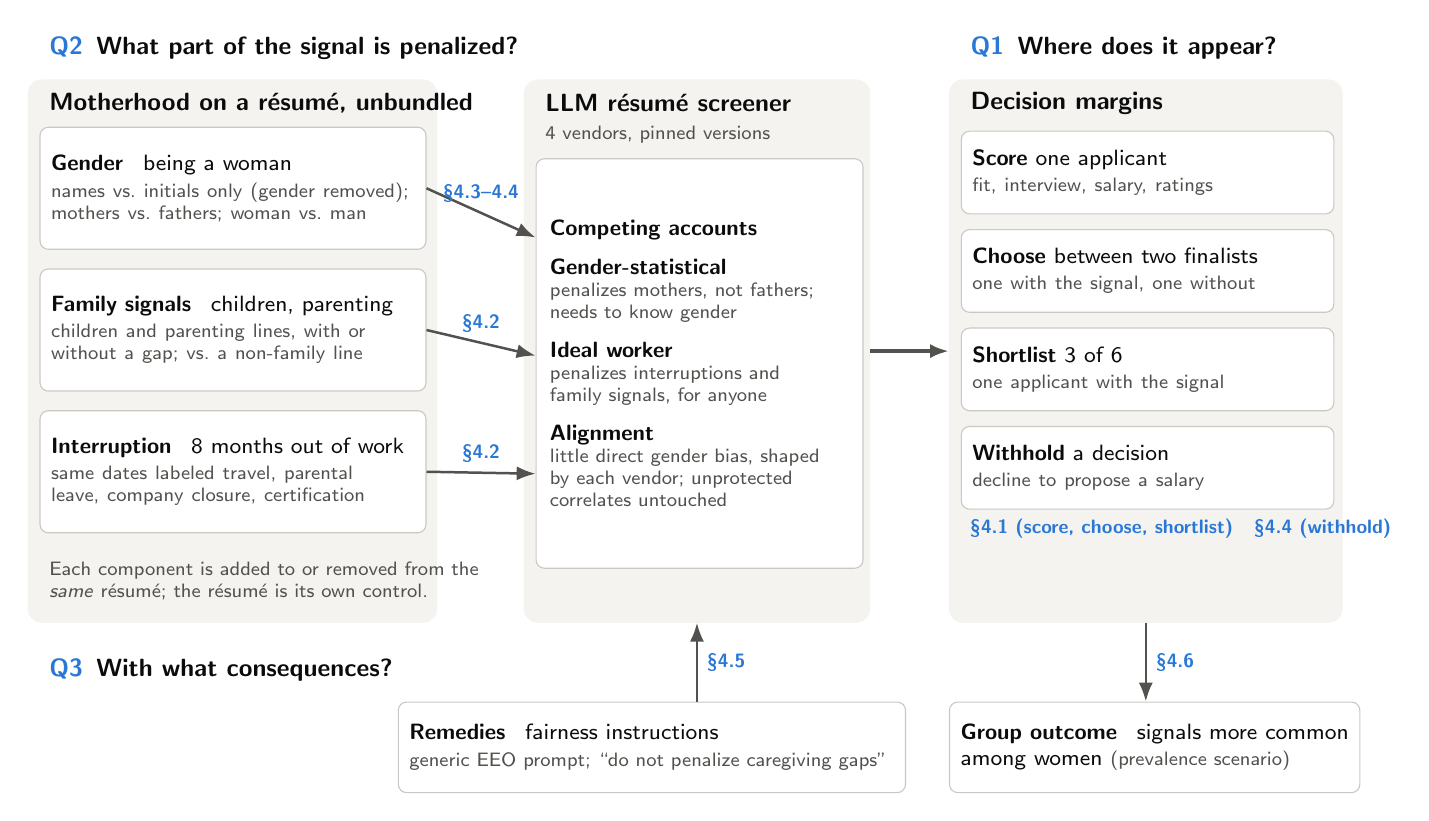
\begin{tikzpicture}[
  font=\footnotesize, color=ink,
  comp/.style={draw=rule, fill=white, rounded corners=3pt, text width=4.62cm, minimum height=1.55cm, align=left, inner sep=4pt, anchor=north west},
  marg/.style={draw=rule, fill=white, rounded corners=3pt, text width=4.45cm, minimum height=1.05cm, align=left, inner sep=4pt, anchor=north west},
  sect/.style={font=\scriptsize\bfseries, text=acc},
  q/.style={font=\small\bfseries, text=ink, anchor=west},
  note/.style={font=\scriptsize, text=ink2, align=left},
  arr/.style={-{Latex[length=2.4mm]}, line width=0.9pt, draw=ink2},
  big/.style={-{Latex[length=3mm]}, line width=2.6pt, draw=acc},
  thin/.style={-{Latex[length=2.2mm]}, line width=0.8pt, draw=ink2, dash pattern=on 2.5pt off 1.5pt},
]
% ---------------- column titles / questions
\node[q] at (0,7.55) {\textcolor{acc}{Q2}\enspace What part of the signal is penalized?};
\node[q] at (11.7,7.55) {\textcolor{acc}{Q1}\enspace Where does it appear?};

% ---------------- A: the unbundled signal
\begin{scope}[on background layer]
\fill[pane, rounded corners=5pt] (-0.15,7.15) rectangle (5.05,0.25);
\end{scope}
\node[font=\small\bfseries, anchor=west] at (0,6.85) {Motherhood on a r\'esum\'e, unbundled};
\node[comp] (G) at (0.0,6.55) {\textbf{Gender} \enspace being a woman\\[2pt]
  \parbox{4.6cm}{\raggedright\scriptsize\color{ink2}names vs.\ initials only (gender removed);\\ mothers vs.\ fathers; woman vs.\ man}};
\node[comp] (F) at (0.0,4.75) {\textbf{Family signals} \enspace children, parenting\\[2pt]
  \parbox{4.6cm}{\raggedright\scriptsize\color{ink2}children and parenting lines, with or\\ without a gap; vs.\ a non-family line}};
\node[comp] (I) at (0.0,2.95) {\textbf{Interruption} \enspace 8 months out of work\\[2pt]
  \parbox{4.6cm}{\raggedright\scriptsize\color{ink2}same dates labeled travel, parental\\ leave, company closure, certification}};
\node[note, anchor=north west] at (0,1.15) {Each component is added to or removed from the\\ \emph{same} r\'esum\'e; the r\'esum\'e is its own control.};

% ---------------- B: the screener
\begin{scope}[on background layer]
\fill[pane, rounded corners=5pt] (6.15,7.15) rectangle (10.55,0.25);
\end{scope}
\node[font=\small\bfseries, anchor=west] at (6.3,6.85) {LLM r\'esum\'e screener};
\node[note, anchor=west] at (6.3,6.45) {4 vendors, pinned versions};
\if\RESULTS0
  \node[draw=rule, fill=white, rounded corners=3pt, anchor=north west, minimum width=4.1cm, minimum height=5.2cm, align=left, inner sep=5pt] (S) at (6.3,6.15) {%
    \parbox{3.8cm}{\textbf{Competing accounts}\\[6pt]
    \textbf{Gender-statistical}\\ \scriptsize\color{ink2} penalizes mothers, not fathers;\\ needs to know gender\\[6pt]
    \normalsize\footnotesize\color{ink}\textbf{Ideal worker}\\ \scriptsize\color{ink2} penalizes interruptions and\\ family signals, for anyone\\[6pt]
    \normalsize\footnotesize\color{ink}\textbf{Alignment}\\ \scriptsize\color{ink2} little direct gender bias, shaped\\ by each vendor; unprotected\\ correlates untouched}};
  \draw[arr] (G.east) -- ($(S.west)+(0,1.6)$) node[midway, above, sect] {\S4.3--4.4};
  \draw[arr] (F.east) -- ($(S.west)+(0,0.1)$) node[midway, above, sect] {\S4.2};
  \draw[arr] (I.east) -- ($(S.west)+(0,-1.4)$) node[midway, above, sect] {\S4.2};
\else
  \node[draw=acc, fill=accl, rounded corners=3pt, anchor=north west, minimum width=4.1cm, minimum height=2.95cm, align=left, inner sep=5pt] (L1) at (6.3,6.15) {%
    \parbox{3.8cm}{\textbf{Layer 1: ideal-worker rule}\\[2pt]\scriptsize gender-blind; same for all vendors in sign\\[3pt]
    \textbullet\ interruption $\to$ availability\\ \phantom{\textbullet\ }inference (instruction reaches it)\\
    \textbullet\ family signals $\to$ norm\\ \phantom{\textbullet\ }(instruction does not)}};
  \node[draw=rule, fill=white, rounded corners=3pt, anchor=north west, minimum width=4.1cm, minimum height=1.9cm, align=left, inner sep=5pt] (L2) at (6.3,2.85) {%
    \parbox{3.8cm}{\textbf{Layer 2: gender layer}\\[2pt]\scriptsize thin; differs by vendor; surfaces\\ when gender is explicit\\ (pro-woman, anti-mother, parity)}};
  \draw[thin] (G.east) -- ($(L2.west)+(0,0.25)$) node[pos=0.18, right, font=\scriptsize, text=ink2] {weak};
  \draw[big] (F.east) -- ($(L1.west)+(0,0.25)$);
  \draw[big] (I.east) -- ($(L1.west)+(0,-0.9)$);
  \node[font=\scriptsize\bfseries, text=acc, anchor=west] at (5.08,2.35) {strong};
\fi

% ---------------- C: decision margins
\begin{scope}[on background layer]
\fill[pane, rounded corners=5pt] (11.55,7.15) rectangle (16.55,0.25);
\end{scope}
\node[font=\small\bfseries, anchor=west] at (11.7,6.85) {Decision margins};
\if\RESULTS0
  \node[marg] (M1) at (11.7,6.5) {\textbf{Score} one applicant\\ \scriptsize\color{ink2}fit, interview, salary, ratings};
  \node[marg] (M2) at (11.7,5.25) {\textbf{Choose} between two finalists\\ \scriptsize\color{ink2}one with the signal, one without};
  \node[marg] (M3) at (11.7,4.0) {\textbf{Shortlist} 3 of 6\\ \scriptsize\color{ink2}one applicant with the signal};
  \node[marg] (M4) at (11.7,2.75) {\textbf{Withhold} a decision\\ \scriptsize\color{ink2}decline to propose a salary};
  \node[sect, anchor=west] at (11.7,1.45) {\S4.1 (score, choose, shortlist)\quad \S4.4 (withhold)};
\else
  \node[marg] (M1) at (11.7,6.5) {\textbf{Score}: \enspace barely moves\\ \scriptsize\color{ink2}$\le$0.35 of 10 fit points};
  \node[marg, draw=acc, line width=0.9pt] (M2) at (11.7,5.25) {\textbf{Choose}: \enspace large penalty\\ \scriptsize\color{ink2}with leave: chosen 11--31\%, not 50\%};
  \node[marg, draw=acc, line width=0.9pt] (M3) at (11.7,4.0) {\textbf{Shortlist}: \enspace large penalty\\ \scriptsize\color{ink2}mothers: 25--78\% of childless rate};
  \node[marg] (M4) at (11.7,2.75) {\textbf{Withhold}: \enspace one vendor\\ \scriptsize\color{ink2}no salary: 20\% of pregnant applicants};
  \node[note, anchor=west] at (11.7,1.45) {Penalty is comparative: invisible to\\ single-applicant scoring audits.};
\fi
\draw[arr, line width=1.6pt] (10.55,3.7) -- (11.55,3.7);

% ---------------- D: consequences
\node[q] at (0,-0.35) {\textcolor{acc}{Q3}\enspace With what consequences?};
\node[draw=rule, fill=white, rounded corners=3pt, anchor=north west, minimum width=6.0cm, minimum height=1.15cm, align=left, inner sep=4pt] (R) at (4.55,-0.75) {%
  \if\RESULTS0 \textbf{Remedies} \enspace fairness instructions\\ \scriptsize\color{ink2}generic EEO prompt; ``do not penalize caregiving gaps''
  \else \textbf{Remedies}: \enspace reach interruption, not family\\ \scriptsize\color{ink2}generic prompt helps, does nothing, or backfires\fi};
\node[draw=rule, fill=white, rounded corners=3pt, anchor=north west, minimum width=5.0cm, minimum height=1.15cm, align=left, inner sep=4pt] (O) at (11.55,-0.75) {%
  \if\RESULTS0 \textbf{Group outcome} \enspace signals more common\\ among women \scriptsize\color{ink2}(prevalence scenario)
  \else \textbf{Group outcome}: \enspace gender-blind rule,\\ gendered result \scriptsize\color{ink2}(Haiku: four-fifths line at 31\%)\fi};
\draw[{Latex[length=2.4mm]}-, line width=0.9pt, draw=ink2] (8.35,0.25) -- (8.35,-0.75) node[pos=0.5, right, sect] {\S4.5};
\draw[arr] (14.05,0.25) -- (14.05,-0.75) node[pos=0.5, right, sect] {\S4.6};
\end{tikzpicture}
\end{document}
"  -> findings view
\documentclass[border=4pt]{standalone}
\usepackage[T1]{fontenc}
\usepackage{helvet}\renewcommand{\familydefault}{\sfdefault}
\usepackage{tikz}
\usetikzlibrary{positioning,arrows.meta,calc,fit,backgrounds}
\ifdefined\RESULTS\else\def\RESULTS{0}\fi
\definecolor{ink}{HTML}{0B0B0B}\definecolor{ink2}{HTML}{52514E}
\definecolor{acc}{HTML}{2A78D6}\definecolor{accl}{HTML}{E3EEFB}
\definecolor{pane}{HTML}{F4F3F0}\definecolor{rule}{HTML}{C9C8C2}
\begin{document}
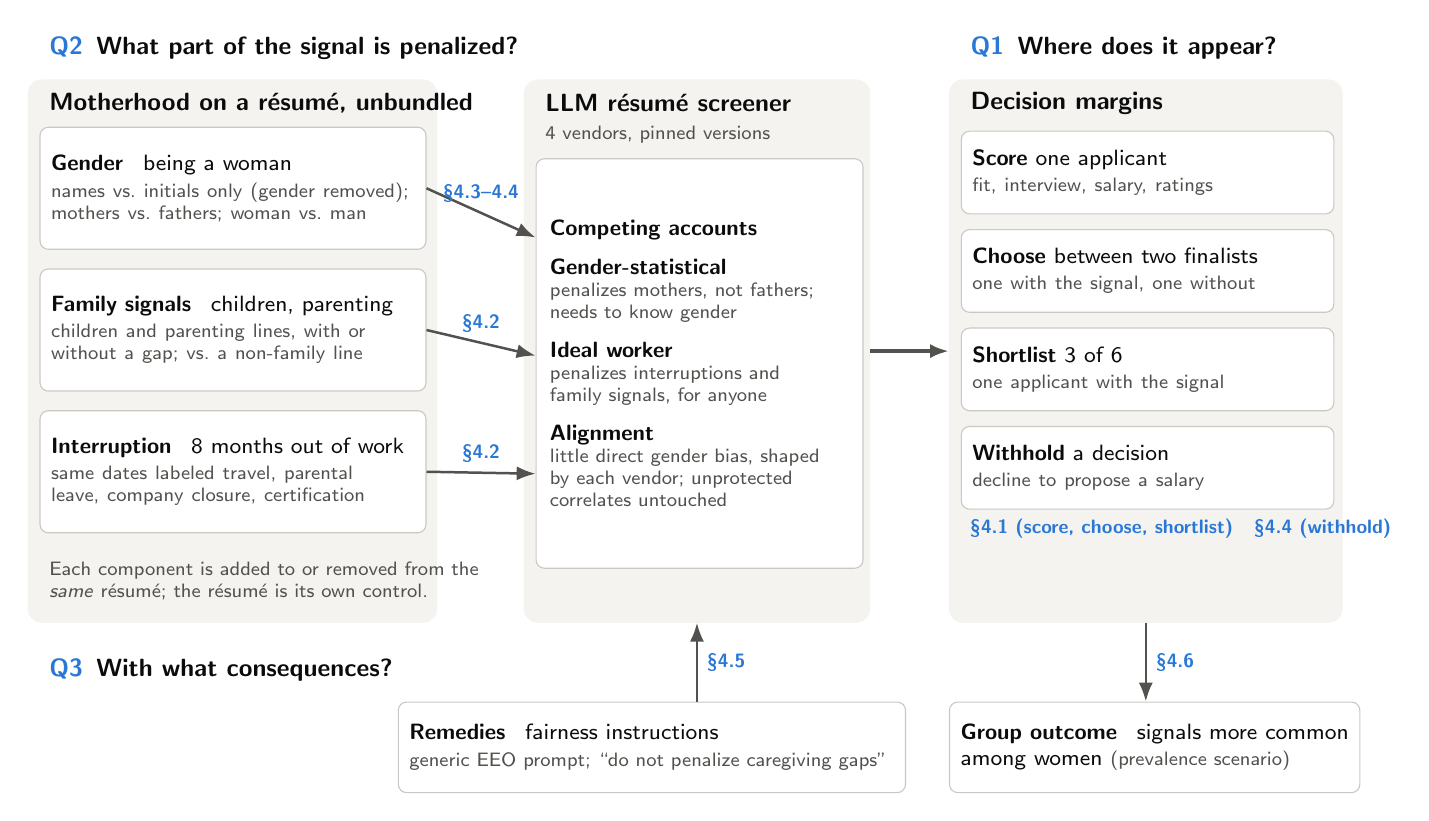
\begin{tikzpicture}[
  font=\footnotesize, color=ink,
  comp/.style={draw=rule, fill=white, rounded corners=3pt, text width=4.62cm, minimum height=1.55cm, align=left, inner sep=4pt, anchor=north west},
  marg/.style={draw=rule, fill=white, rounded corners=3pt, text width=4.45cm, minimum height=1.05cm, align=left, inner sep=4pt, anchor=north west},
  sect/.style={font=\scriptsize\bfseries, text=acc},
  q/.style={font=\small\bfseries, text=ink, anchor=west},
  note/.style={font=\scriptsize, text=ink2, align=left},
  arr/.style={-{Latex[length=2.4mm]}, line width=0.9pt, draw=ink2},
  big/.style={-{Latex[length=3mm]}, line width=2.6pt, draw=acc},
  thin/.style={-{Latex[length=2.2mm]}, line width=0.8pt, draw=ink2, dash pattern=on 2.5pt off 1.5pt},
]
% ---------------- column titles / questions
\node[q] at (0,7.55) {\textcolor{acc}{Q2}\enspace What part of the signal is penalized?};
\node[q] at (11.7,7.55) {\textcolor{acc}{Q1}\enspace Where does it appear?};

% ---------------- A: the unbundled signal
\begin{scope}[on background layer]
\fill[pane, rounded corners=5pt] (-0.15,7.15) rectangle (5.05,0.25);
\end{scope}
\node[font=\small\bfseries, anchor=west] at (0,6.85) {Motherhood on a r\'esum\'e, unbundled};
\node[comp] (G) at (0.0,6.55) {\textbf{Gender} \enspace being a woman\\[2pt]
  \parbox{4.6cm}{\raggedright\scriptsize\color{ink2}names vs.\ initials only (gender removed);\\ mothers vs.\ fathers; woman vs.\ man}};
\node[comp] (F) at (0.0,4.75) {\textbf{Family signals} \enspace children, parenting\\[2pt]
  \parbox{4.6cm}{\raggedright\scriptsize\color{ink2}children and parenting lines, with or\\ without a gap; vs.\ a non-family line}};
\node[comp] (I) at (0.0,2.95) {\textbf{Interruption} \enspace 8 months out of work\\[2pt]
  \parbox{4.6cm}{\raggedright\scriptsize\color{ink2}same dates labeled travel, parental\\ leave, company closure, certification}};
\node[note, anchor=north west] at (0,1.15) {Each component is added to or removed from the\\ \emph{same} r\'esum\'e; the r\'esum\'e is its own control.};

% ---------------- B: the screener
\begin{scope}[on background layer]
\fill[pane, rounded corners=5pt] (6.15,7.15) rectangle (10.55,0.25);
\end{scope}
\node[font=\small\bfseries, anchor=west] at (6.3,6.85) {LLM r\'esum\'e screener};
\node[note, anchor=west] at (6.3,6.45) {4 vendors, pinned versions};
\if\RESULTS0
  \node[draw=rule, fill=white, rounded corners=3pt, anchor=north west, minimum width=4.1cm, minimum height=5.2cm, align=left, inner sep=5pt] (S) at (6.3,6.15) {%
    \parbox{3.8cm}{\textbf{Competing accounts}\\[6pt]
    \textbf{Gender-statistical}\\ \scriptsize\color{ink2} penalizes mothers, not fathers;\\ needs to know gender\\[6pt]
    \normalsize\footnotesize\color{ink}\textbf{Ideal worker}\\ \scriptsize\color{ink2} penalizes interruptions and\\ family signals, for anyone\\[6pt]
    \normalsize\footnotesize\color{ink}\textbf{Alignment}\\ \scriptsize\color{ink2} little direct gender bias, shaped\\ by each vendor; unprotected\\ correlates untouched}};
  \draw[arr] (G.east) -- ($(S.west)+(0,1.6)$) node[midway, above, sect] {\S4.3--4.4};
  \draw[arr] (F.east) -- ($(S.west)+(0,0.1)$) node[midway, above, sect] {\S4.2};
  \draw[arr] (I.east) -- ($(S.west)+(0,-1.4)$) node[midway, above, sect] {\S4.2};
\else
  \node[draw=acc, fill=accl, rounded corners=3pt, anchor=north west, minimum width=4.1cm, minimum height=2.95cm, align=left, inner sep=5pt] (L1) at (6.3,6.15) {%
    \parbox{3.8cm}{\textbf{Layer 1: ideal-worker rule}\\[2pt]\scriptsize gender-blind; same for all vendors in sign\\[3pt]
    \textbullet\ interruption $\to$ availability\\ \phantom{\textbullet\ }inference (instruction reaches it)\\
    \textbullet\ family signals $\to$ norm\\ \phantom{\textbullet\ }(instruction does not)}};
  \node[draw=rule, fill=white, rounded corners=3pt, anchor=north west, minimum width=4.1cm, minimum height=1.9cm, align=left, inner sep=5pt] (L2) at (6.3,2.85) {%
    \parbox{3.8cm}{\textbf{Layer 2: gender layer}\\[2pt]\scriptsize thin; differs by vendor; surfaces\\ when gender is explicit\\ (pro-woman, anti-mother, parity)}};
  \draw[thin] (G.east) -- ($(L2.west)+(0,0.25)$) node[pos=0.18, right, font=\scriptsize, text=ink2] {weak};
  \draw[big] (F.east) -- ($(L1.west)+(0,0.25)$);
  \draw[big] (I.east) -- ($(L1.west)+(0,-0.9)$);
  \node[font=\scriptsize\bfseries, text=acc, anchor=west] at (5.08,2.35) {strong};
\fi

% ---------------- C: decision margins
\begin{scope}[on background layer]
\fill[pane, rounded corners=5pt] (11.55,7.15) rectangle (16.55,0.25);
\end{scope}
\node[font=\small\bfseries, anchor=west] at (11.7,6.85) {Decision margins};
\if\RESULTS0
  \node[marg] (M1) at (11.7,6.5) {\textbf{Score} one applicant\\ \scriptsize\color{ink2}fit, interview, salary, ratings};
  \node[marg] (M2) at (11.7,5.25) {\textbf{Choose} between two finalists\\ \scriptsize\color{ink2}one with the signal, one without};
  \node[marg] (M3) at (11.7,4.0) {\textbf{Shortlist} 3 of 6\\ \scriptsize\color{ink2}one applicant with the signal};
  \node[marg] (M4) at (11.7,2.75) {\textbf{Withhold} a decision\\ \scriptsize\color{ink2}decline to propose a salary};
  \node[sect, anchor=west] at (11.7,1.45) {\S4.1 (score, choose, shortlist)\quad \S4.4 (withhold)};
\else
  \node[marg] (M1) at (11.7,6.5) {\textbf{Score}: \enspace barely moves\\ \scriptsize\color{ink2}$\le$0.35 of 10 fit points};
  \node[marg, draw=acc, line width=0.9pt] (M2) at (11.7,5.25) {\textbf{Choose}: \enspace large penalty\\ \scriptsize\color{ink2}with leave: chosen 11--31\%, not 50\%};
  \node[marg, draw=acc, line width=0.9pt] (M3) at (11.7,4.0) {\textbf{Shortlist}: \enspace large penalty\\ \scriptsize\color{ink2}mothers: 25--78\% of childless rate};
  \node[marg] (M4) at (11.7,2.75) {\textbf{Withhold}: \enspace one vendor\\ \scriptsize\color{ink2}no salary: 20\% of pregnant applicants};
  \node[note, anchor=west] at (11.7,1.45) {Penalty is comparative: invisible to\\ single-applicant scoring audits.};
\fi
\draw[arr, line width=1.6pt] (10.55,3.7) -- (11.55,3.7);

% ---------------- D: consequences
\node[q] at (0,-0.35) {\textcolor{acc}{Q3}\enspace With what consequences?};
\node[draw=rule, fill=white, rounded corners=3pt, anchor=north west, minimum width=6.0cm, minimum height=1.15cm, align=left, inner sep=4pt] (R) at (4.55,-0.75) {%
  \if\RESULTS0 \textbf{Remedies} \enspace fairness instructions\\ \scriptsize\color{ink2}generic EEO prompt; ``do not penalize caregiving gaps''
  \else \textbf{Remedies}: \enspace reach interruption, not family\\ \scriptsize\color{ink2}generic prompt helps, does nothing, or backfires\fi};
\node[draw=rule, fill=white, rounded corners=3pt, anchor=north west, minimum width=5.0cm, minimum height=1.15cm, align=left, inner sep=4pt] (O) at (11.55,-0.75) {%
  \if\RESULTS0 \textbf{Group outcome} \enspace signals more common\\ among women \scriptsize\color{ink2}(prevalence scenario)
  \else \textbf{Group outcome}: \enspace gender-blind rule,\\ gendered result \scriptsize\color{ink2}(Haiku: four-fifths line at 31\%)\fi};
\draw[{Latex[length=2.4mm]}-, line width=0.9pt, draw=ink2] (8.35,0.25) -- (8.35,-0.75) node[pos=0.5, right, sect] {\S4.5};
\draw[arr] (14.05,0.25) -- (14.05,-0.75) node[pos=0.5, right, sect] {\S4.6};
\end{tikzpicture}
\end{document}
"  -> framework view
%          pdflatex "\def\RESULTS{1}% Figure 1 (framework) and Figure 9 (findings mapped onto the same framework).
% Compile: pdflatex "\def\RESULTS{0}% Figure 1 (framework) and Figure 9 (findings mapped onto the same framework).
% Compile: pdflatex "\def\RESULTS{0}\input{framework}"  -> framework view
%          pdflatex "\def\RESULTS{1}\input{framework}"  -> findings view
\documentclass[border=4pt]{standalone}
\usepackage[T1]{fontenc}
\usepackage{helvet}\renewcommand{\familydefault}{\sfdefault}
\usepackage{tikz}
\usetikzlibrary{positioning,arrows.meta,calc,fit,backgrounds}
\ifdefined\RESULTS\else\def\RESULTS{0}\fi
\definecolor{ink}{HTML}{0B0B0B}\definecolor{ink2}{HTML}{52514E}
\definecolor{acc}{HTML}{2A78D6}\definecolor{accl}{HTML}{E3EEFB}
\definecolor{pane}{HTML}{F4F3F0}\definecolor{rule}{HTML}{C9C8C2}
\begin{document}
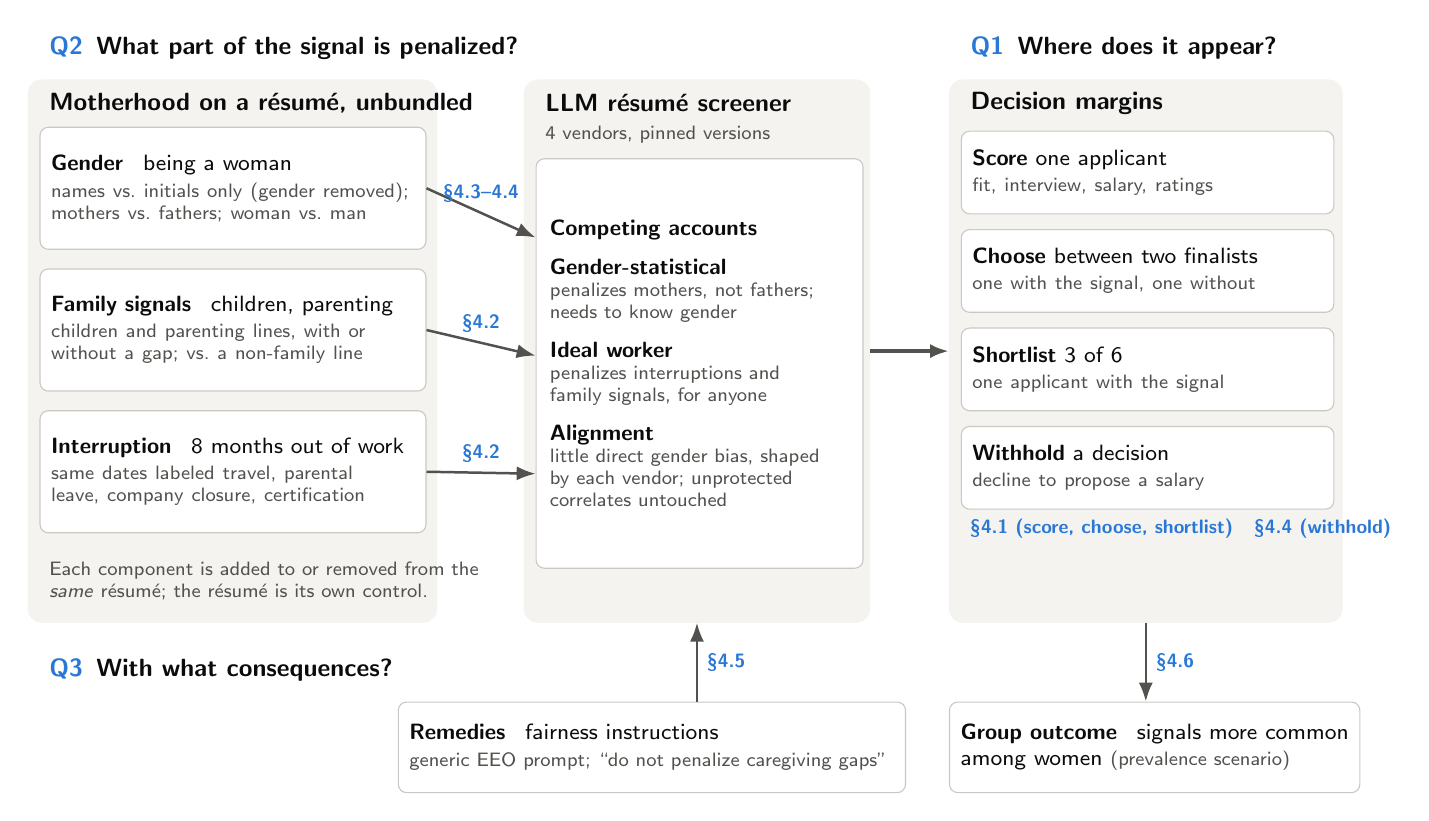
\begin{tikzpicture}[
  font=\footnotesize, color=ink,
  comp/.style={draw=rule, fill=white, rounded corners=3pt, text width=4.62cm, minimum height=1.55cm, align=left, inner sep=4pt, anchor=north west},
  marg/.style={draw=rule, fill=white, rounded corners=3pt, text width=4.45cm, minimum height=1.05cm, align=left, inner sep=4pt, anchor=north west},
  sect/.style={font=\scriptsize\bfseries, text=acc},
  q/.style={font=\small\bfseries, text=ink, anchor=west},
  note/.style={font=\scriptsize, text=ink2, align=left},
  arr/.style={-{Latex[length=2.4mm]}, line width=0.9pt, draw=ink2},
  big/.style={-{Latex[length=3mm]}, line width=2.6pt, draw=acc},
  thin/.style={-{Latex[length=2.2mm]}, line width=0.8pt, draw=ink2, dash pattern=on 2.5pt off 1.5pt},
]
% ---------------- column titles / questions
\node[q] at (0,7.55) {\textcolor{acc}{Q2}\enspace What part of the signal is penalized?};
\node[q] at (11.7,7.55) {\textcolor{acc}{Q1}\enspace Where does it appear?};

% ---------------- A: the unbundled signal
\begin{scope}[on background layer]
\fill[pane, rounded corners=5pt] (-0.15,7.15) rectangle (5.05,0.25);
\end{scope}
\node[font=\small\bfseries, anchor=west] at (0,6.85) {Motherhood on a r\'esum\'e, unbundled};
\node[comp] (G) at (0.0,6.55) {\textbf{Gender} \enspace being a woman\\[2pt]
  \parbox{4.6cm}{\raggedright\scriptsize\color{ink2}names vs.\ initials only (gender removed);\\ mothers vs.\ fathers; woman vs.\ man}};
\node[comp] (F) at (0.0,4.75) {\textbf{Family signals} \enspace children, parenting\\[2pt]
  \parbox{4.6cm}{\raggedright\scriptsize\color{ink2}children and parenting lines, with or\\ without a gap; vs.\ a non-family line}};
\node[comp] (I) at (0.0,2.95) {\textbf{Interruption} \enspace 8 months out of work\\[2pt]
  \parbox{4.6cm}{\raggedright\scriptsize\color{ink2}same dates labeled travel, parental\\ leave, company closure, certification}};
\node[note, anchor=north west] at (0,1.15) {Each component is added to or removed from the\\ \emph{same} r\'esum\'e; the r\'esum\'e is its own control.};

% ---------------- B: the screener
\begin{scope}[on background layer]
\fill[pane, rounded corners=5pt] (6.15,7.15) rectangle (10.55,0.25);
\end{scope}
\node[font=\small\bfseries, anchor=west] at (6.3,6.85) {LLM r\'esum\'e screener};
\node[note, anchor=west] at (6.3,6.45) {4 vendors, pinned versions};
\if\RESULTS0
  \node[draw=rule, fill=white, rounded corners=3pt, anchor=north west, minimum width=4.1cm, minimum height=5.2cm, align=left, inner sep=5pt] (S) at (6.3,6.15) {%
    \parbox{3.8cm}{\textbf{Competing accounts}\\[6pt]
    \textbf{Gender-statistical}\\ \scriptsize\color{ink2} penalizes mothers, not fathers;\\ needs to know gender\\[6pt]
    \normalsize\footnotesize\color{ink}\textbf{Ideal worker}\\ \scriptsize\color{ink2} penalizes interruptions and\\ family signals, for anyone\\[6pt]
    \normalsize\footnotesize\color{ink}\textbf{Alignment}\\ \scriptsize\color{ink2} little direct gender bias, shaped\\ by each vendor; unprotected\\ correlates untouched}};
  \draw[arr] (G.east) -- ($(S.west)+(0,1.6)$) node[midway, above, sect] {\S4.3--4.4};
  \draw[arr] (F.east) -- ($(S.west)+(0,0.1)$) node[midway, above, sect] {\S4.2};
  \draw[arr] (I.east) -- ($(S.west)+(0,-1.4)$) node[midway, above, sect] {\S4.2};
\else
  \node[draw=acc, fill=accl, rounded corners=3pt, anchor=north west, minimum width=4.1cm, minimum height=2.95cm, align=left, inner sep=5pt] (L1) at (6.3,6.15) {%
    \parbox{3.8cm}{\textbf{Layer 1: ideal-worker rule}\\[2pt]\scriptsize gender-blind; same for all vendors in sign\\[3pt]
    \textbullet\ interruption $\to$ availability\\ \phantom{\textbullet\ }inference (instruction reaches it)\\
    \textbullet\ family signals $\to$ norm\\ \phantom{\textbullet\ }(instruction does not)}};
  \node[draw=rule, fill=white, rounded corners=3pt, anchor=north west, minimum width=4.1cm, minimum height=1.9cm, align=left, inner sep=5pt] (L2) at (6.3,2.85) {%
    \parbox{3.8cm}{\textbf{Layer 2: gender layer}\\[2pt]\scriptsize thin; differs by vendor; surfaces\\ when gender is explicit\\ (pro-woman, anti-mother, parity)}};
  \draw[thin] (G.east) -- ($(L2.west)+(0,0.25)$) node[pos=0.18, right, font=\scriptsize, text=ink2] {weak};
  \draw[big] (F.east) -- ($(L1.west)+(0,0.25)$);
  \draw[big] (I.east) -- ($(L1.west)+(0,-0.9)$);
  \node[font=\scriptsize\bfseries, text=acc, anchor=west] at (5.08,2.35) {strong};
\fi

% ---------------- C: decision margins
\begin{scope}[on background layer]
\fill[pane, rounded corners=5pt] (11.55,7.15) rectangle (16.55,0.25);
\end{scope}
\node[font=\small\bfseries, anchor=west] at (11.7,6.85) {Decision margins};
\if\RESULTS0
  \node[marg] (M1) at (11.7,6.5) {\textbf{Score} one applicant\\ \scriptsize\color{ink2}fit, interview, salary, ratings};
  \node[marg] (M2) at (11.7,5.25) {\textbf{Choose} between two finalists\\ \scriptsize\color{ink2}one with the signal, one without};
  \node[marg] (M3) at (11.7,4.0) {\textbf{Shortlist} 3 of 6\\ \scriptsize\color{ink2}one applicant with the signal};
  \node[marg] (M4) at (11.7,2.75) {\textbf{Withhold} a decision\\ \scriptsize\color{ink2}decline to propose a salary};
  \node[sect, anchor=west] at (11.7,1.45) {\S4.1 (score, choose, shortlist)\quad \S4.4 (withhold)};
\else
  \node[marg] (M1) at (11.7,6.5) {\textbf{Score}: \enspace barely moves\\ \scriptsize\color{ink2}$\le$0.35 of 10 fit points};
  \node[marg, draw=acc, line width=0.9pt] (M2) at (11.7,5.25) {\textbf{Choose}: \enspace large penalty\\ \scriptsize\color{ink2}with leave: chosen 11--31\%, not 50\%};
  \node[marg, draw=acc, line width=0.9pt] (M3) at (11.7,4.0) {\textbf{Shortlist}: \enspace large penalty\\ \scriptsize\color{ink2}mothers: 25--78\% of childless rate};
  \node[marg] (M4) at (11.7,2.75) {\textbf{Withhold}: \enspace one vendor\\ \scriptsize\color{ink2}no salary: 20\% of pregnant applicants};
  \node[note, anchor=west] at (11.7,1.45) {Penalty is comparative: invisible to\\ single-applicant scoring audits.};
\fi
\draw[arr, line width=1.6pt] (10.55,3.7) -- (11.55,3.7);

% ---------------- D: consequences
\node[q] at (0,-0.35) {\textcolor{acc}{Q3}\enspace With what consequences?};
\node[draw=rule, fill=white, rounded corners=3pt, anchor=north west, minimum width=6.0cm, minimum height=1.15cm, align=left, inner sep=4pt] (R) at (4.55,-0.75) {%
  \if\RESULTS0 \textbf{Remedies} \enspace fairness instructions\\ \scriptsize\color{ink2}generic EEO prompt; ``do not penalize caregiving gaps''
  \else \textbf{Remedies}: \enspace reach interruption, not family\\ \scriptsize\color{ink2}generic prompt helps, does nothing, or backfires\fi};
\node[draw=rule, fill=white, rounded corners=3pt, anchor=north west, minimum width=5.0cm, minimum height=1.15cm, align=left, inner sep=4pt] (O) at (11.55,-0.75) {%
  \if\RESULTS0 \textbf{Group outcome} \enspace signals more common\\ among women \scriptsize\color{ink2}(prevalence scenario)
  \else \textbf{Group outcome}: \enspace gender-blind rule,\\ gendered result \scriptsize\color{ink2}(Haiku: four-fifths line at 31\%)\fi};
\draw[{Latex[length=2.4mm]}-, line width=0.9pt, draw=ink2] (8.35,0.25) -- (8.35,-0.75) node[pos=0.5, right, sect] {\S4.5};
\draw[arr] (14.05,0.25) -- (14.05,-0.75) node[pos=0.5, right, sect] {\S4.6};
\end{tikzpicture}
\end{document}
"  -> framework view
%          pdflatex "\def\RESULTS{1}% Figure 1 (framework) and Figure 9 (findings mapped onto the same framework).
% Compile: pdflatex "\def\RESULTS{0}\input{framework}"  -> framework view
%          pdflatex "\def\RESULTS{1}\input{framework}"  -> findings view
\documentclass[border=4pt]{standalone}
\usepackage[T1]{fontenc}
\usepackage{helvet}\renewcommand{\familydefault}{\sfdefault}
\usepackage{tikz}
\usetikzlibrary{positioning,arrows.meta,calc,fit,backgrounds}
\ifdefined\RESULTS\else\def\RESULTS{0}\fi
\definecolor{ink}{HTML}{0B0B0B}\definecolor{ink2}{HTML}{52514E}
\definecolor{acc}{HTML}{2A78D6}\definecolor{accl}{HTML}{E3EEFB}
\definecolor{pane}{HTML}{F4F3F0}\definecolor{rule}{HTML}{C9C8C2}
\begin{document}
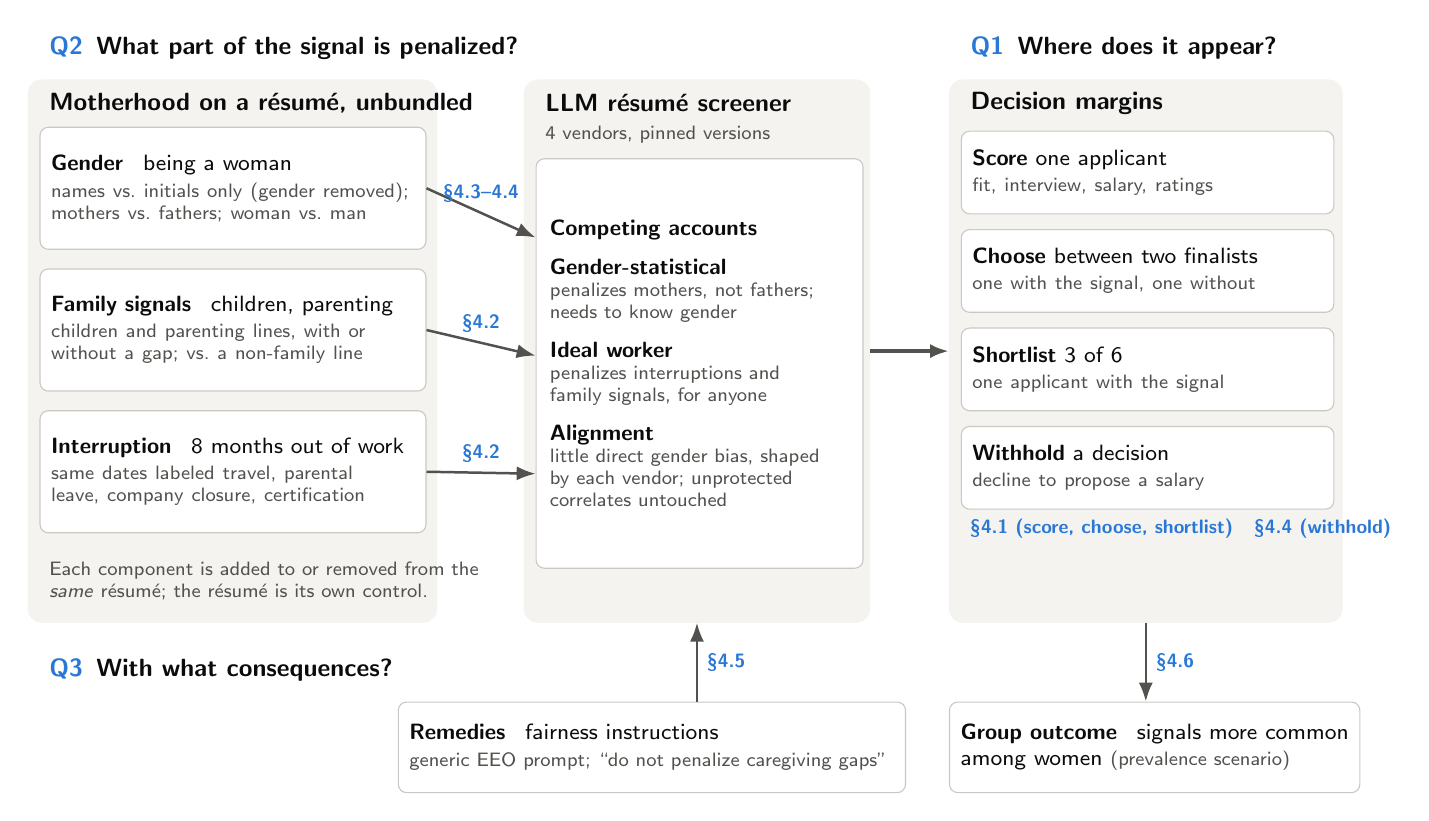
\begin{tikzpicture}[
  font=\footnotesize, color=ink,
  comp/.style={draw=rule, fill=white, rounded corners=3pt, text width=4.62cm, minimum height=1.55cm, align=left, inner sep=4pt, anchor=north west},
  marg/.style={draw=rule, fill=white, rounded corners=3pt, text width=4.45cm, minimum height=1.05cm, align=left, inner sep=4pt, anchor=north west},
  sect/.style={font=\scriptsize\bfseries, text=acc},
  q/.style={font=\small\bfseries, text=ink, anchor=west},
  note/.style={font=\scriptsize, text=ink2, align=left},
  arr/.style={-{Latex[length=2.4mm]}, line width=0.9pt, draw=ink2},
  big/.style={-{Latex[length=3mm]}, line width=2.6pt, draw=acc},
  thin/.style={-{Latex[length=2.2mm]}, line width=0.8pt, draw=ink2, dash pattern=on 2.5pt off 1.5pt},
]
% ---------------- column titles / questions
\node[q] at (0,7.55) {\textcolor{acc}{Q2}\enspace What part of the signal is penalized?};
\node[q] at (11.7,7.55) {\textcolor{acc}{Q1}\enspace Where does it appear?};

% ---------------- A: the unbundled signal
\begin{scope}[on background layer]
\fill[pane, rounded corners=5pt] (-0.15,7.15) rectangle (5.05,0.25);
\end{scope}
\node[font=\small\bfseries, anchor=west] at (0,6.85) {Motherhood on a r\'esum\'e, unbundled};
\node[comp] (G) at (0.0,6.55) {\textbf{Gender} \enspace being a woman\\[2pt]
  \parbox{4.6cm}{\raggedright\scriptsize\color{ink2}names vs.\ initials only (gender removed);\\ mothers vs.\ fathers; woman vs.\ man}};
\node[comp] (F) at (0.0,4.75) {\textbf{Family signals} \enspace children, parenting\\[2pt]
  \parbox{4.6cm}{\raggedright\scriptsize\color{ink2}children and parenting lines, with or\\ without a gap; vs.\ a non-family line}};
\node[comp] (I) at (0.0,2.95) {\textbf{Interruption} \enspace 8 months out of work\\[2pt]
  \parbox{4.6cm}{\raggedright\scriptsize\color{ink2}same dates labeled travel, parental\\ leave, company closure, certification}};
\node[note, anchor=north west] at (0,1.15) {Each component is added to or removed from the\\ \emph{same} r\'esum\'e; the r\'esum\'e is its own control.};

% ---------------- B: the screener
\begin{scope}[on background layer]
\fill[pane, rounded corners=5pt] (6.15,7.15) rectangle (10.55,0.25);
\end{scope}
\node[font=\small\bfseries, anchor=west] at (6.3,6.85) {LLM r\'esum\'e screener};
\node[note, anchor=west] at (6.3,6.45) {4 vendors, pinned versions};
\if\RESULTS0
  \node[draw=rule, fill=white, rounded corners=3pt, anchor=north west, minimum width=4.1cm, minimum height=5.2cm, align=left, inner sep=5pt] (S) at (6.3,6.15) {%
    \parbox{3.8cm}{\textbf{Competing accounts}\\[6pt]
    \textbf{Gender-statistical}\\ \scriptsize\color{ink2} penalizes mothers, not fathers;\\ needs to know gender\\[6pt]
    \normalsize\footnotesize\color{ink}\textbf{Ideal worker}\\ \scriptsize\color{ink2} penalizes interruptions and\\ family signals, for anyone\\[6pt]
    \normalsize\footnotesize\color{ink}\textbf{Alignment}\\ \scriptsize\color{ink2} little direct gender bias, shaped\\ by each vendor; unprotected\\ correlates untouched}};
  \draw[arr] (G.east) -- ($(S.west)+(0,1.6)$) node[midway, above, sect] {\S4.3--4.4};
  \draw[arr] (F.east) -- ($(S.west)+(0,0.1)$) node[midway, above, sect] {\S4.2};
  \draw[arr] (I.east) -- ($(S.west)+(0,-1.4)$) node[midway, above, sect] {\S4.2};
\else
  \node[draw=acc, fill=accl, rounded corners=3pt, anchor=north west, minimum width=4.1cm, minimum height=2.95cm, align=left, inner sep=5pt] (L1) at (6.3,6.15) {%
    \parbox{3.8cm}{\textbf{Layer 1: ideal-worker rule}\\[2pt]\scriptsize gender-blind; same for all vendors in sign\\[3pt]
    \textbullet\ interruption $\to$ availability\\ \phantom{\textbullet\ }inference (instruction reaches it)\\
    \textbullet\ family signals $\to$ norm\\ \phantom{\textbullet\ }(instruction does not)}};
  \node[draw=rule, fill=white, rounded corners=3pt, anchor=north west, minimum width=4.1cm, minimum height=1.9cm, align=left, inner sep=5pt] (L2) at (6.3,2.85) {%
    \parbox{3.8cm}{\textbf{Layer 2: gender layer}\\[2pt]\scriptsize thin; differs by vendor; surfaces\\ when gender is explicit\\ (pro-woman, anti-mother, parity)}};
  \draw[thin] (G.east) -- ($(L2.west)+(0,0.25)$) node[pos=0.18, right, font=\scriptsize, text=ink2] {weak};
  \draw[big] (F.east) -- ($(L1.west)+(0,0.25)$);
  \draw[big] (I.east) -- ($(L1.west)+(0,-0.9)$);
  \node[font=\scriptsize\bfseries, text=acc, anchor=west] at (5.08,2.35) {strong};
\fi

% ---------------- C: decision margins
\begin{scope}[on background layer]
\fill[pane, rounded corners=5pt] (11.55,7.15) rectangle (16.55,0.25);
\end{scope}
\node[font=\small\bfseries, anchor=west] at (11.7,6.85) {Decision margins};
\if\RESULTS0
  \node[marg] (M1) at (11.7,6.5) {\textbf{Score} one applicant\\ \scriptsize\color{ink2}fit, interview, salary, ratings};
  \node[marg] (M2) at (11.7,5.25) {\textbf{Choose} between two finalists\\ \scriptsize\color{ink2}one with the signal, one without};
  \node[marg] (M3) at (11.7,4.0) {\textbf{Shortlist} 3 of 6\\ \scriptsize\color{ink2}one applicant with the signal};
  \node[marg] (M4) at (11.7,2.75) {\textbf{Withhold} a decision\\ \scriptsize\color{ink2}decline to propose a salary};
  \node[sect, anchor=west] at (11.7,1.45) {\S4.1 (score, choose, shortlist)\quad \S4.4 (withhold)};
\else
  \node[marg] (M1) at (11.7,6.5) {\textbf{Score}: \enspace barely moves\\ \scriptsize\color{ink2}$\le$0.35 of 10 fit points};
  \node[marg, draw=acc, line width=0.9pt] (M2) at (11.7,5.25) {\textbf{Choose}: \enspace large penalty\\ \scriptsize\color{ink2}with leave: chosen 11--31\%, not 50\%};
  \node[marg, draw=acc, line width=0.9pt] (M3) at (11.7,4.0) {\textbf{Shortlist}: \enspace large penalty\\ \scriptsize\color{ink2}mothers: 25--78\% of childless rate};
  \node[marg] (M4) at (11.7,2.75) {\textbf{Withhold}: \enspace one vendor\\ \scriptsize\color{ink2}no salary: 20\% of pregnant applicants};
  \node[note, anchor=west] at (11.7,1.45) {Penalty is comparative: invisible to\\ single-applicant scoring audits.};
\fi
\draw[arr, line width=1.6pt] (10.55,3.7) -- (11.55,3.7);

% ---------------- D: consequences
\node[q] at (0,-0.35) {\textcolor{acc}{Q3}\enspace With what consequences?};
\node[draw=rule, fill=white, rounded corners=3pt, anchor=north west, minimum width=6.0cm, minimum height=1.15cm, align=left, inner sep=4pt] (R) at (4.55,-0.75) {%
  \if\RESULTS0 \textbf{Remedies} \enspace fairness instructions\\ \scriptsize\color{ink2}generic EEO prompt; ``do not penalize caregiving gaps''
  \else \textbf{Remedies}: \enspace reach interruption, not family\\ \scriptsize\color{ink2}generic prompt helps, does nothing, or backfires\fi};
\node[draw=rule, fill=white, rounded corners=3pt, anchor=north west, minimum width=5.0cm, minimum height=1.15cm, align=left, inner sep=4pt] (O) at (11.55,-0.75) {%
  \if\RESULTS0 \textbf{Group outcome} \enspace signals more common\\ among women \scriptsize\color{ink2}(prevalence scenario)
  \else \textbf{Group outcome}: \enspace gender-blind rule,\\ gendered result \scriptsize\color{ink2}(Haiku: four-fifths line at 31\%)\fi};
\draw[{Latex[length=2.4mm]}-, line width=0.9pt, draw=ink2] (8.35,0.25) -- (8.35,-0.75) node[pos=0.5, right, sect] {\S4.5};
\draw[arr] (14.05,0.25) -- (14.05,-0.75) node[pos=0.5, right, sect] {\S4.6};
\end{tikzpicture}
\end{document}
"  -> findings view
\documentclass[border=4pt]{standalone}
\usepackage[T1]{fontenc}
\usepackage{helvet}\renewcommand{\familydefault}{\sfdefault}
\usepackage{tikz}
\usetikzlibrary{positioning,arrows.meta,calc,fit,backgrounds}
\ifdefined\RESULTS\else\def\RESULTS{0}\fi
\definecolor{ink}{HTML}{0B0B0B}\definecolor{ink2}{HTML}{52514E}
\definecolor{acc}{HTML}{2A78D6}\definecolor{accl}{HTML}{E3EEFB}
\definecolor{pane}{HTML}{F4F3F0}\definecolor{rule}{HTML}{C9C8C2}
\begin{document}
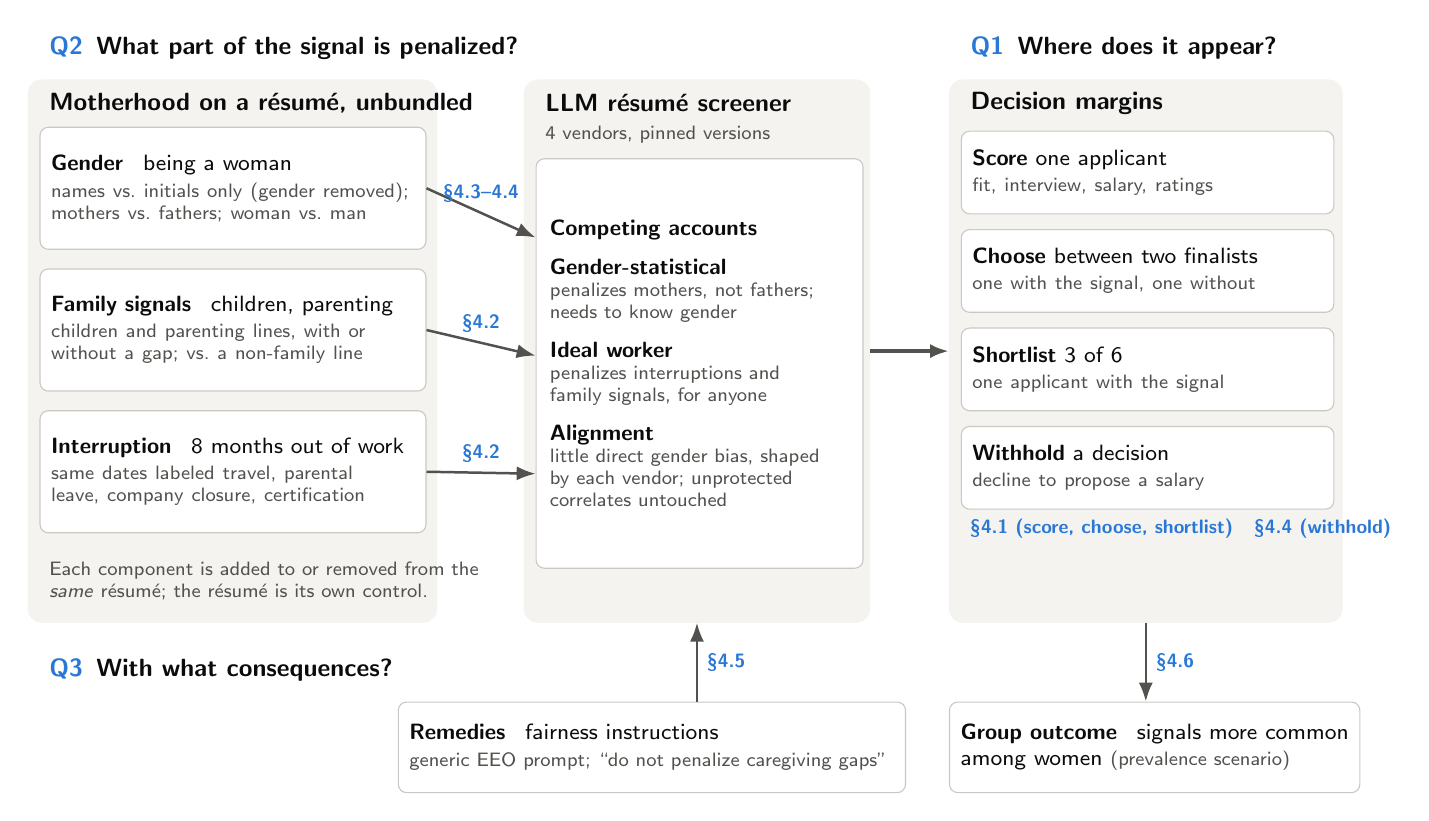
\begin{tikzpicture}[
  font=\footnotesize, color=ink,
  comp/.style={draw=rule, fill=white, rounded corners=3pt, text width=4.62cm, minimum height=1.55cm, align=left, inner sep=4pt, anchor=north west},
  marg/.style={draw=rule, fill=white, rounded corners=3pt, text width=4.45cm, minimum height=1.05cm, align=left, inner sep=4pt, anchor=north west},
  sect/.style={font=\scriptsize\bfseries, text=acc},
  q/.style={font=\small\bfseries, text=ink, anchor=west},
  note/.style={font=\scriptsize, text=ink2, align=left},
  arr/.style={-{Latex[length=2.4mm]}, line width=0.9pt, draw=ink2},
  big/.style={-{Latex[length=3mm]}, line width=2.6pt, draw=acc},
  thin/.style={-{Latex[length=2.2mm]}, line width=0.8pt, draw=ink2, dash pattern=on 2.5pt off 1.5pt},
]
% ---------------- column titles / questions
\node[q] at (0,7.55) {\textcolor{acc}{Q2}\enspace What part of the signal is penalized?};
\node[q] at (11.7,7.55) {\textcolor{acc}{Q1}\enspace Where does it appear?};

% ---------------- A: the unbundled signal
\begin{scope}[on background layer]
\fill[pane, rounded corners=5pt] (-0.15,7.15) rectangle (5.05,0.25);
\end{scope}
\node[font=\small\bfseries, anchor=west] at (0,6.85) {Motherhood on a r\'esum\'e, unbundled};
\node[comp] (G) at (0.0,6.55) {\textbf{Gender} \enspace being a woman\\[2pt]
  \parbox{4.6cm}{\raggedright\scriptsize\color{ink2}names vs.\ initials only (gender removed);\\ mothers vs.\ fathers; woman vs.\ man}};
\node[comp] (F) at (0.0,4.75) {\textbf{Family signals} \enspace children, parenting\\[2pt]
  \parbox{4.6cm}{\raggedright\scriptsize\color{ink2}children and parenting lines, with or\\ without a gap; vs.\ a non-family line}};
\node[comp] (I) at (0.0,2.95) {\textbf{Interruption} \enspace 8 months out of work\\[2pt]
  \parbox{4.6cm}{\raggedright\scriptsize\color{ink2}same dates labeled travel, parental\\ leave, company closure, certification}};
\node[note, anchor=north west] at (0,1.15) {Each component is added to or removed from the\\ \emph{same} r\'esum\'e; the r\'esum\'e is its own control.};

% ---------------- B: the screener
\begin{scope}[on background layer]
\fill[pane, rounded corners=5pt] (6.15,7.15) rectangle (10.55,0.25);
\end{scope}
\node[font=\small\bfseries, anchor=west] at (6.3,6.85) {LLM r\'esum\'e screener};
\node[note, anchor=west] at (6.3,6.45) {4 vendors, pinned versions};
\if\RESULTS0
  \node[draw=rule, fill=white, rounded corners=3pt, anchor=north west, minimum width=4.1cm, minimum height=5.2cm, align=left, inner sep=5pt] (S) at (6.3,6.15) {%
    \parbox{3.8cm}{\textbf{Competing accounts}\\[6pt]
    \textbf{Gender-statistical}\\ \scriptsize\color{ink2} penalizes mothers, not fathers;\\ needs to know gender\\[6pt]
    \normalsize\footnotesize\color{ink}\textbf{Ideal worker}\\ \scriptsize\color{ink2} penalizes interruptions and\\ family signals, for anyone\\[6pt]
    \normalsize\footnotesize\color{ink}\textbf{Alignment}\\ \scriptsize\color{ink2} little direct gender bias, shaped\\ by each vendor; unprotected\\ correlates untouched}};
  \draw[arr] (G.east) -- ($(S.west)+(0,1.6)$) node[midway, above, sect] {\S4.3--4.4};
  \draw[arr] (F.east) -- ($(S.west)+(0,0.1)$) node[midway, above, sect] {\S4.2};
  \draw[arr] (I.east) -- ($(S.west)+(0,-1.4)$) node[midway, above, sect] {\S4.2};
\else
  \node[draw=acc, fill=accl, rounded corners=3pt, anchor=north west, minimum width=4.1cm, minimum height=2.95cm, align=left, inner sep=5pt] (L1) at (6.3,6.15) {%
    \parbox{3.8cm}{\textbf{Layer 1: ideal-worker rule}\\[2pt]\scriptsize gender-blind; same for all vendors in sign\\[3pt]
    \textbullet\ interruption $\to$ availability\\ \phantom{\textbullet\ }inference (instruction reaches it)\\
    \textbullet\ family signals $\to$ norm\\ \phantom{\textbullet\ }(instruction does not)}};
  \node[draw=rule, fill=white, rounded corners=3pt, anchor=north west, minimum width=4.1cm, minimum height=1.9cm, align=left, inner sep=5pt] (L2) at (6.3,2.85) {%
    \parbox{3.8cm}{\textbf{Layer 2: gender layer}\\[2pt]\scriptsize thin; differs by vendor; surfaces\\ when gender is explicit\\ (pro-woman, anti-mother, parity)}};
  \draw[thin] (G.east) -- ($(L2.west)+(0,0.25)$) node[pos=0.18, right, font=\scriptsize, text=ink2] {weak};
  \draw[big] (F.east) -- ($(L1.west)+(0,0.25)$);
  \draw[big] (I.east) -- ($(L1.west)+(0,-0.9)$);
  \node[font=\scriptsize\bfseries, text=acc, anchor=west] at (5.08,2.35) {strong};
\fi

% ---------------- C: decision margins
\begin{scope}[on background layer]
\fill[pane, rounded corners=5pt] (11.55,7.15) rectangle (16.55,0.25);
\end{scope}
\node[font=\small\bfseries, anchor=west] at (11.7,6.85) {Decision margins};
\if\RESULTS0
  \node[marg] (M1) at (11.7,6.5) {\textbf{Score} one applicant\\ \scriptsize\color{ink2}fit, interview, salary, ratings};
  \node[marg] (M2) at (11.7,5.25) {\textbf{Choose} between two finalists\\ \scriptsize\color{ink2}one with the signal, one without};
  \node[marg] (M3) at (11.7,4.0) {\textbf{Shortlist} 3 of 6\\ \scriptsize\color{ink2}one applicant with the signal};
  \node[marg] (M4) at (11.7,2.75) {\textbf{Withhold} a decision\\ \scriptsize\color{ink2}decline to propose a salary};
  \node[sect, anchor=west] at (11.7,1.45) {\S4.1 (score, choose, shortlist)\quad \S4.4 (withhold)};
\else
  \node[marg] (M1) at (11.7,6.5) {\textbf{Score}: \enspace barely moves\\ \scriptsize\color{ink2}$\le$0.35 of 10 fit points};
  \node[marg, draw=acc, line width=0.9pt] (M2) at (11.7,5.25) {\textbf{Choose}: \enspace large penalty\\ \scriptsize\color{ink2}with leave: chosen 11--31\%, not 50\%};
  \node[marg, draw=acc, line width=0.9pt] (M3) at (11.7,4.0) {\textbf{Shortlist}: \enspace large penalty\\ \scriptsize\color{ink2}mothers: 25--78\% of childless rate};
  \node[marg] (M4) at (11.7,2.75) {\textbf{Withhold}: \enspace one vendor\\ \scriptsize\color{ink2}no salary: 20\% of pregnant applicants};
  \node[note, anchor=west] at (11.7,1.45) {Penalty is comparative: invisible to\\ single-applicant scoring audits.};
\fi
\draw[arr, line width=1.6pt] (10.55,3.7) -- (11.55,3.7);

% ---------------- D: consequences
\node[q] at (0,-0.35) {\textcolor{acc}{Q3}\enspace With what consequences?};
\node[draw=rule, fill=white, rounded corners=3pt, anchor=north west, minimum width=6.0cm, minimum height=1.15cm, align=left, inner sep=4pt] (R) at (4.55,-0.75) {%
  \if\RESULTS0 \textbf{Remedies} \enspace fairness instructions\\ \scriptsize\color{ink2}generic EEO prompt; ``do not penalize caregiving gaps''
  \else \textbf{Remedies}: \enspace reach interruption, not family\\ \scriptsize\color{ink2}generic prompt helps, does nothing, or backfires\fi};
\node[draw=rule, fill=white, rounded corners=3pt, anchor=north west, minimum width=5.0cm, minimum height=1.15cm, align=left, inner sep=4pt] (O) at (11.55,-0.75) {%
  \if\RESULTS0 \textbf{Group outcome} \enspace signals more common\\ among women \scriptsize\color{ink2}(prevalence scenario)
  \else \textbf{Group outcome}: \enspace gender-blind rule,\\ gendered result \scriptsize\color{ink2}(Haiku: four-fifths line at 31\%)\fi};
\draw[{Latex[length=2.4mm]}-, line width=0.9pt, draw=ink2] (8.35,0.25) -- (8.35,-0.75) node[pos=0.5, right, sect] {\S4.5};
\draw[arr] (14.05,0.25) -- (14.05,-0.75) node[pos=0.5, right, sect] {\S4.6};
\end{tikzpicture}
\end{document}
"  -> findings view
\documentclass[border=4pt]{standalone}
\usepackage[T1]{fontenc}
\usepackage{helvet}\renewcommand{\familydefault}{\sfdefault}
\usepackage{tikz}
\usetikzlibrary{positioning,arrows.meta,calc,fit,backgrounds}
\ifdefined\RESULTS\else\def\RESULTS{0}\fi
\definecolor{ink}{HTML}{0B0B0B}\definecolor{ink2}{HTML}{52514E}
\definecolor{acc}{HTML}{2A78D6}\definecolor{accl}{HTML}{E3EEFB}
\definecolor{pane}{HTML}{F4F3F0}\definecolor{rule}{HTML}{C9C8C2}
\begin{document}
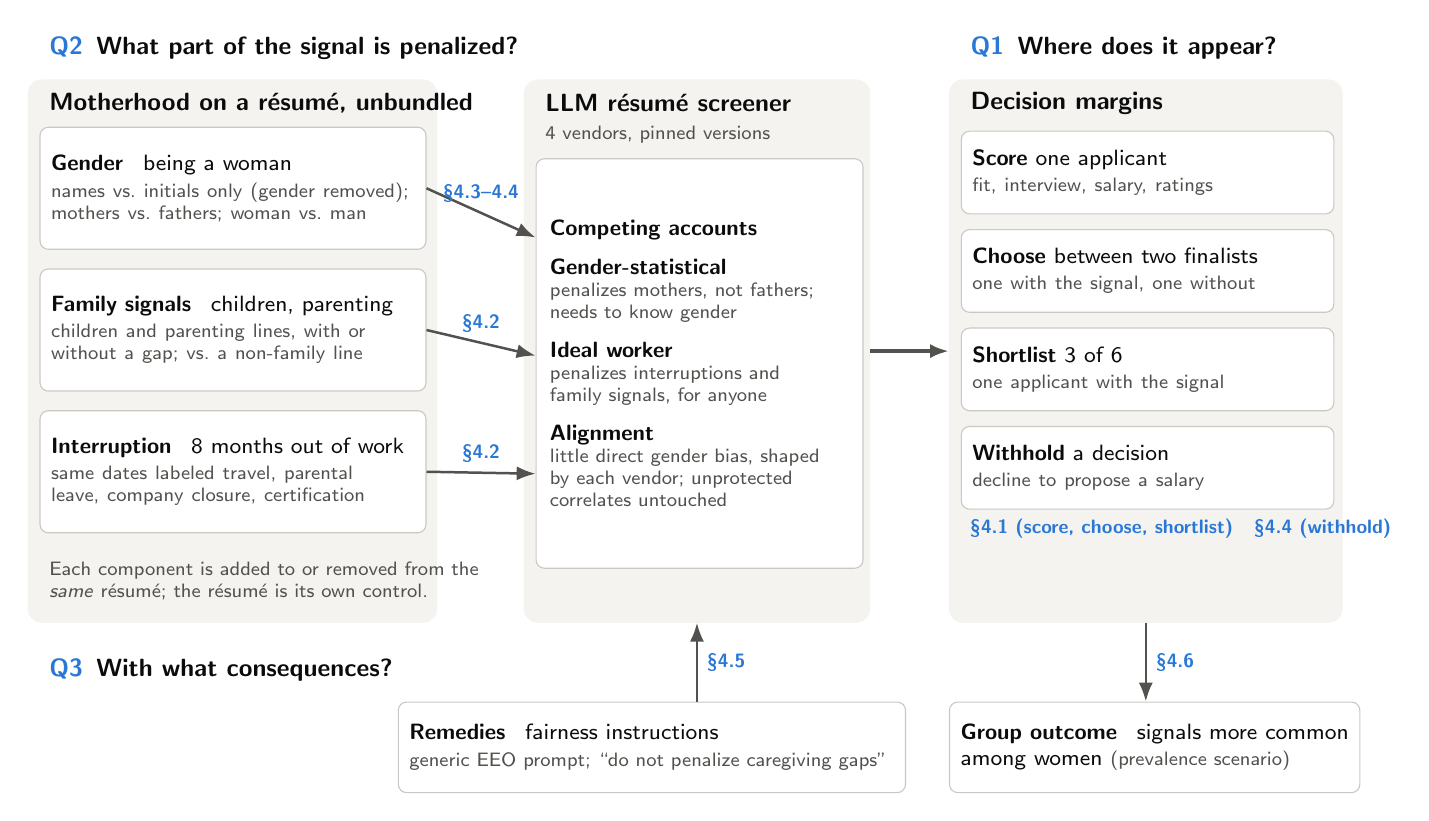
\begin{tikzpicture}[
  font=\footnotesize, color=ink,
  comp/.style={draw=rule, fill=white, rounded corners=3pt, text width=4.62cm, minimum height=1.55cm, align=left, inner sep=4pt, anchor=north west},
  marg/.style={draw=rule, fill=white, rounded corners=3pt, text width=4.45cm, minimum height=1.05cm, align=left, inner sep=4pt, anchor=north west},
  sect/.style={font=\scriptsize\bfseries, text=acc},
  q/.style={font=\small\bfseries, text=ink, anchor=west},
  note/.style={font=\scriptsize, text=ink2, align=left},
  arr/.style={-{Latex[length=2.4mm]}, line width=0.9pt, draw=ink2},
  big/.style={-{Latex[length=3mm]}, line width=2.6pt, draw=acc},
  thin/.style={-{Latex[length=2.2mm]}, line width=0.8pt, draw=ink2, dash pattern=on 2.5pt off 1.5pt},
]
% ---------------- column titles / questions
\node[q] at (0,7.55) {\textcolor{acc}{Q2}\enspace What part of the signal is penalized?};
\node[q] at (11.7,7.55) {\textcolor{acc}{Q1}\enspace Where does it appear?};

% ---------------- A: the unbundled signal
\begin{scope}[on background layer]
\fill[pane, rounded corners=5pt] (-0.15,7.15) rectangle (5.05,0.25);
\end{scope}
\node[font=\small\bfseries, anchor=west] at (0,6.85) {Motherhood on a r\'esum\'e, unbundled};
\node[comp] (G) at (0.0,6.55) {\textbf{Gender} \enspace being a woman\\[2pt]
  \parbox{4.6cm}{\raggedright\scriptsize\color{ink2}names vs.\ initials only (gender removed);\\ mothers vs.\ fathers; woman vs.\ man}};
\node[comp] (F) at (0.0,4.75) {\textbf{Family signals} \enspace children, parenting\\[2pt]
  \parbox{4.6cm}{\raggedright\scriptsize\color{ink2}children and parenting lines, with or\\ without a gap; vs.\ a non-family line}};
\node[comp] (I) at (0.0,2.95) {\textbf{Interruption} \enspace 8 months out of work\\[2pt]
  \parbox{4.6cm}{\raggedright\scriptsize\color{ink2}same dates labeled travel, parental\\ leave, company closure, certification}};
\node[note, anchor=north west] at (0,1.15) {Each component is added to or removed from the\\ \emph{same} r\'esum\'e; the r\'esum\'e is its own control.};

% ---------------- B: the screener
\begin{scope}[on background layer]
\fill[pane, rounded corners=5pt] (6.15,7.15) rectangle (10.55,0.25);
\end{scope}
\node[font=\small\bfseries, anchor=west] at (6.3,6.85) {LLM r\'esum\'e screener};
\node[note, anchor=west] at (6.3,6.45) {4 vendors, pinned versions};
\if\RESULTS0
  \node[draw=rule, fill=white, rounded corners=3pt, anchor=north west, minimum width=4.1cm, minimum height=5.2cm, align=left, inner sep=5pt] (S) at (6.3,6.15) {%
    \parbox{3.8cm}{\textbf{Competing accounts}\\[6pt]
    \textbf{Gender-statistical}\\ \scriptsize\color{ink2} penalizes mothers, not fathers;\\ needs to know gender\\[6pt]
    \normalsize\footnotesize\color{ink}\textbf{Ideal worker}\\ \scriptsize\color{ink2} penalizes interruptions and\\ family signals, for anyone\\[6pt]
    \normalsize\footnotesize\color{ink}\textbf{Alignment}\\ \scriptsize\color{ink2} little direct gender bias, shaped\\ by each vendor; unprotected\\ correlates untouched}};
  \draw[arr] (G.east) -- ($(S.west)+(0,1.6)$) node[midway, above, sect] {\S4.3--4.4};
  \draw[arr] (F.east) -- ($(S.west)+(0,0.1)$) node[midway, above, sect] {\S4.2};
  \draw[arr] (I.east) -- ($(S.west)+(0,-1.4)$) node[midway, above, sect] {\S4.2};
\else
  \node[draw=acc, fill=accl, rounded corners=3pt, anchor=north west, minimum width=4.1cm, minimum height=2.95cm, align=left, inner sep=5pt] (L1) at (6.3,6.15) {%
    \parbox{3.8cm}{\textbf{Layer 1: ideal-worker rule}\\[2pt]\scriptsize gender-blind; same for all vendors in sign\\[3pt]
    \textbullet\ interruption $\to$ availability\\ \phantom{\textbullet\ }inference (instruction reaches it)\\
    \textbullet\ family signals $\to$ norm\\ \phantom{\textbullet\ }(instruction does not)}};
  \node[draw=rule, fill=white, rounded corners=3pt, anchor=north west, minimum width=4.1cm, minimum height=1.9cm, align=left, inner sep=5pt] (L2) at (6.3,2.85) {%
    \parbox{3.8cm}{\textbf{Layer 2: gender layer}\\[2pt]\scriptsize thin; differs by vendor; surfaces\\ when gender is explicit\\ (pro-woman, anti-mother, parity)}};
  \draw[thin] (G.east) -- ($(L2.west)+(0,0.25)$) node[pos=0.18, right, font=\scriptsize, text=ink2] {weak};
  \draw[big] (F.east) -- ($(L1.west)+(0,0.25)$);
  \draw[big] (I.east) -- ($(L1.west)+(0,-0.9)$);
  \node[font=\scriptsize\bfseries, text=acc, anchor=west] at (5.08,2.35) {strong};
\fi

% ---------------- C: decision margins
\begin{scope}[on background layer]
\fill[pane, rounded corners=5pt] (11.55,7.15) rectangle (16.55,0.25);
\end{scope}
\node[font=\small\bfseries, anchor=west] at (11.7,6.85) {Decision margins};
\if\RESULTS0
  \node[marg] (M1) at (11.7,6.5) {\textbf{Score} one applicant\\ \scriptsize\color{ink2}fit, interview, salary, ratings};
  \node[marg] (M2) at (11.7,5.25) {\textbf{Choose} between two finalists\\ \scriptsize\color{ink2}one with the signal, one without};
  \node[marg] (M3) at (11.7,4.0) {\textbf{Shortlist} 3 of 6\\ \scriptsize\color{ink2}one applicant with the signal};
  \node[marg] (M4) at (11.7,2.75) {\textbf{Withhold} a decision\\ \scriptsize\color{ink2}decline to propose a salary};
  \node[sect, anchor=west] at (11.7,1.45) {\S4.1 (score, choose, shortlist)\quad \S4.4 (withhold)};
\else
  \node[marg] (M1) at (11.7,6.5) {\textbf{Score}: \enspace barely moves\\ \scriptsize\color{ink2}$\le$0.35 of 10 fit points};
  \node[marg, draw=acc, line width=0.9pt] (M2) at (11.7,5.25) {\textbf{Choose}: \enspace large penalty\\ \scriptsize\color{ink2}with leave: chosen 11--31\%, not 50\%};
  \node[marg, draw=acc, line width=0.9pt] (M3) at (11.7,4.0) {\textbf{Shortlist}: \enspace large penalty\\ \scriptsize\color{ink2}mothers: 25--78\% of childless rate};
  \node[marg] (M4) at (11.7,2.75) {\textbf{Withhold}: \enspace one vendor\\ \scriptsize\color{ink2}no salary: 20\% of pregnant applicants};
  \node[note, anchor=west] at (11.7,1.45) {Penalty is comparative: invisible to\\ single-applicant scoring audits.};
\fi
\draw[arr, line width=1.6pt] (10.55,3.7) -- (11.55,3.7);

% ---------------- D: consequences
\node[q] at (0,-0.35) {\textcolor{acc}{Q3}\enspace With what consequences?};
\node[draw=rule, fill=white, rounded corners=3pt, anchor=north west, minimum width=6.0cm, minimum height=1.15cm, align=left, inner sep=4pt] (R) at (4.55,-0.75) {%
  \if\RESULTS0 \textbf{Remedies} \enspace fairness instructions\\ \scriptsize\color{ink2}generic EEO prompt; ``do not penalize caregiving gaps''
  \else \textbf{Remedies}: \enspace reach interruption, not family\\ \scriptsize\color{ink2}generic prompt helps, does nothing, or backfires\fi};
\node[draw=rule, fill=white, rounded corners=3pt, anchor=north west, minimum width=5.0cm, minimum height=1.15cm, align=left, inner sep=4pt] (O) at (11.55,-0.75) {%
  \if\RESULTS0 \textbf{Group outcome} \enspace signals more common\\ among women \scriptsize\color{ink2}(prevalence scenario)
  \else \textbf{Group outcome}: \enspace gender-blind rule,\\ gendered result \scriptsize\color{ink2}(Haiku: four-fifths line at 31\%)\fi};
\draw[{Latex[length=2.4mm]}-, line width=0.9pt, draw=ink2] (8.35,0.25) -- (8.35,-0.75) node[pos=0.5, right, sect] {\S4.5};
\draw[arr] (14.05,0.25) -- (14.05,-0.75) node[pos=0.5, right, sect] {\S4.6};
\end{tikzpicture}
\end{document}
"  -> findings view
\documentclass[border=4pt]{standalone}
\usepackage[T1]{fontenc}
\usepackage{helvet}\renewcommand{\familydefault}{\sfdefault}
\usepackage{tikz}
\usetikzlibrary{positioning,arrows.meta,calc,fit,backgrounds}
\ifdefined\RESULTS\else\def\RESULTS{0}\fi
\definecolor{ink}{HTML}{0B0B0B}\definecolor{ink2}{HTML}{52514E}
\definecolor{acc}{HTML}{2A78D6}\definecolor{accl}{HTML}{E3EEFB}
\definecolor{pane}{HTML}{F4F3F0}\definecolor{rule}{HTML}{C9C8C2}
\begin{document}
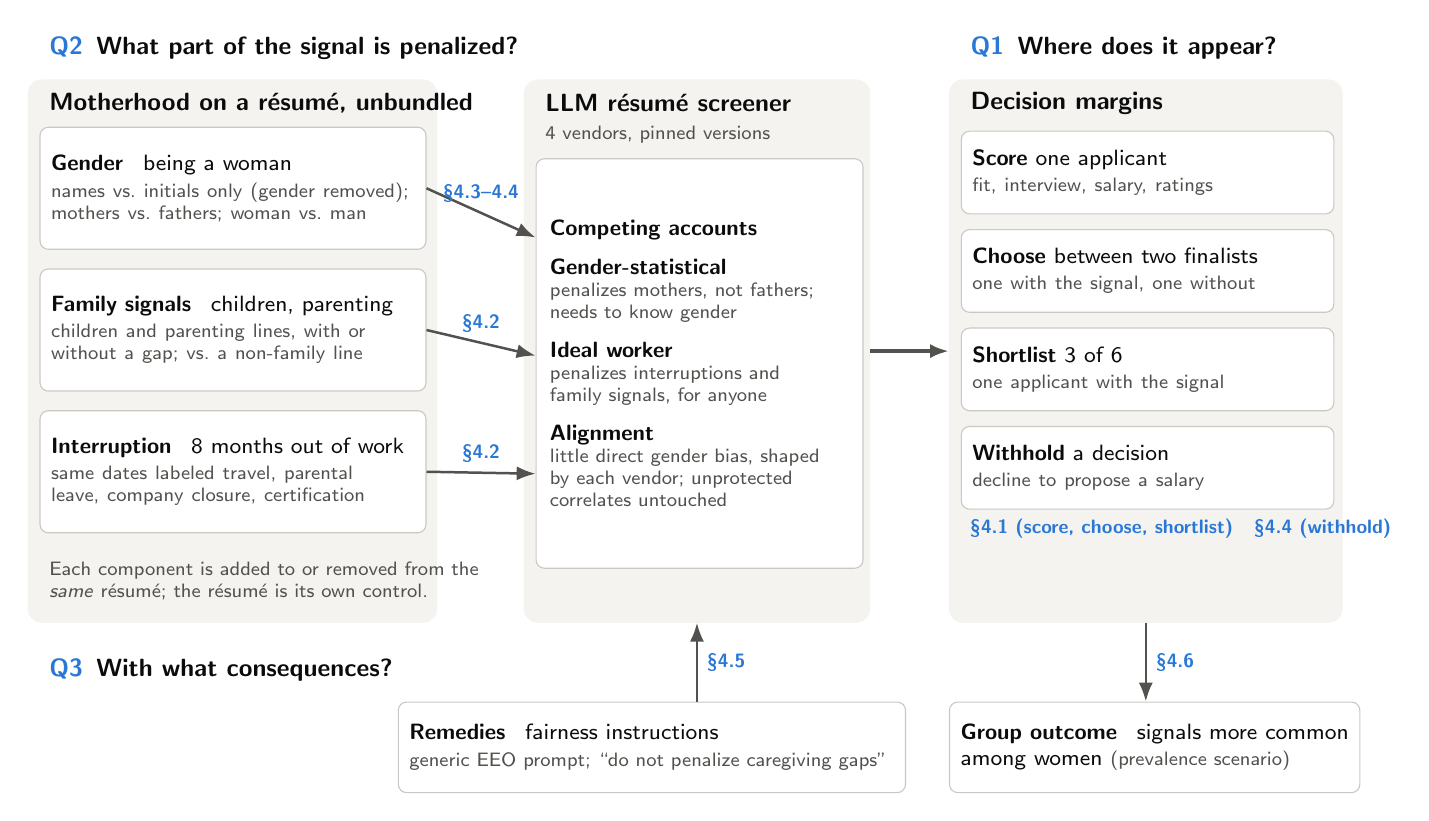
\begin{tikzpicture}[
  font=\footnotesize, color=ink,
  comp/.style={draw=rule, fill=white, rounded corners=3pt, text width=4.62cm, minimum height=1.55cm, align=left, inner sep=4pt, anchor=north west},
  marg/.style={draw=rule, fill=white, rounded corners=3pt, text width=4.45cm, minimum height=1.05cm, align=left, inner sep=4pt, anchor=north west},
  sect/.style={font=\scriptsize\bfseries, text=acc},
  q/.style={font=\small\bfseries, text=ink, anchor=west},
  note/.style={font=\scriptsize, text=ink2, align=left},
  arr/.style={-{Latex[length=2.4mm]}, line width=0.9pt, draw=ink2},
  big/.style={-{Latex[length=3mm]}, line width=2.6pt, draw=acc},
  thin/.style={-{Latex[length=2.2mm]}, line width=0.8pt, draw=ink2, dash pattern=on 2.5pt off 1.5pt},
]
% ---------------- column titles / questions
\node[q] at (0,7.55) {\textcolor{acc}{Q2}\enspace What part of the signal is penalized?};
\node[q] at (11.7,7.55) {\textcolor{acc}{Q1}\enspace Where does it appear?};

% ---------------- A: the unbundled signal
\begin{scope}[on background layer]
\fill[pane, rounded corners=5pt] (-0.15,7.15) rectangle (5.05,0.25);
\end{scope}
\node[font=\small\bfseries, anchor=west] at (0,6.85) {Motherhood on a r\'esum\'e, unbundled};
\node[comp] (G) at (0.0,6.55) {\textbf{Gender} \enspace being a woman\\[2pt]
  \parbox{4.6cm}{\raggedright\scriptsize\color{ink2}names vs.\ initials only (gender removed);\\ mothers vs.\ fathers; woman vs.\ man}};
\node[comp] (F) at (0.0,4.75) {\textbf{Family signals} \enspace children, parenting\\[2pt]
  \parbox{4.6cm}{\raggedright\scriptsize\color{ink2}children and parenting lines, with or\\ without a gap; vs.\ a non-family line}};
\node[comp] (I) at (0.0,2.95) {\textbf{Interruption} \enspace 8 months out of work\\[2pt]
  \parbox{4.6cm}{\raggedright\scriptsize\color{ink2}same dates labeled travel, parental\\ leave, company closure, certification}};
\node[note, anchor=north west] at (0,1.15) {Each component is added to or removed from the\\ \emph{same} r\'esum\'e; the r\'esum\'e is its own control.};

% ---------------- B: the screener
\begin{scope}[on background layer]
\fill[pane, rounded corners=5pt] (6.15,7.15) rectangle (10.55,0.25);
\end{scope}
\node[font=\small\bfseries, anchor=west] at (6.3,6.85) {LLM r\'esum\'e screener};
\node[note, anchor=west] at (6.3,6.45) {4 vendors, pinned versions};
\if\RESULTS0
  \node[draw=rule, fill=white, rounded corners=3pt, anchor=north west, minimum width=4.1cm, minimum height=5.2cm, align=left, inner sep=5pt] (S) at (6.3,6.15) {%
    \parbox{3.8cm}{\textbf{Competing accounts}\\[6pt]
    \textbf{Gender-statistical}\\ \scriptsize\color{ink2} penalizes mothers, not fathers;\\ needs to know gender\\[6pt]
    \normalsize\footnotesize\color{ink}\textbf{Ideal worker}\\ \scriptsize\color{ink2} penalizes interruptions and\\ family signals, for anyone\\[6pt]
    \normalsize\footnotesize\color{ink}\textbf{Alignment}\\ \scriptsize\color{ink2} little direct gender bias, shaped\\ by each vendor; unprotected\\ correlates untouched}};
  \draw[arr] (G.east) -- ($(S.west)+(0,1.6)$) node[midway, above, sect] {\S4.3--4.4};
  \draw[arr] (F.east) -- ($(S.west)+(0,0.1)$) node[midway, above, sect] {\S4.2};
  \draw[arr] (I.east) -- ($(S.west)+(0,-1.4)$) node[midway, above, sect] {\S4.2};
\else
  \node[draw=acc, fill=accl, rounded corners=3pt, anchor=north west, minimum width=4.1cm, minimum height=2.95cm, align=left, inner sep=5pt] (L1) at (6.3,6.15) {%
    \parbox{3.8cm}{\textbf{Layer 1: ideal-worker rule}\\[2pt]\scriptsize gender-blind; same for all vendors in sign\\[3pt]
    \textbullet\ interruption $\to$ availability\\ \phantom{\textbullet\ }inference (instruction reaches it)\\
    \textbullet\ family signals $\to$ norm\\ \phantom{\textbullet\ }(instruction does not)}};
  \node[draw=rule, fill=white, rounded corners=3pt, anchor=north west, minimum width=4.1cm, minimum height=1.9cm, align=left, inner sep=5pt] (L2) at (6.3,2.85) {%
    \parbox{3.8cm}{\textbf{Layer 2: gender layer}\\[2pt]\scriptsize thin; differs by vendor; surfaces\\ when gender is explicit\\ (pro-woman, anti-mother, parity)}};
  \draw[thin] (G.east) -- ($(L2.west)+(0,0.25)$) node[pos=0.18, right, font=\scriptsize, text=ink2] {weak};
  \draw[big] (F.east) -- ($(L1.west)+(0,0.25)$);
  \draw[big] (I.east) -- ($(L1.west)+(0,-0.9)$);
  \node[font=\scriptsize\bfseries, text=acc, anchor=west] at (5.08,2.35) {strong};
\fi

% ---------------- C: decision margins
\begin{scope}[on background layer]
\fill[pane, rounded corners=5pt] (11.55,7.15) rectangle (16.55,0.25);
\end{scope}
\node[font=\small\bfseries, anchor=west] at (11.7,6.85) {Decision margins};
\if\RESULTS0
  \node[marg] (M1) at (11.7,6.5) {\textbf{Score} one applicant\\ \scriptsize\color{ink2}fit, interview, salary, ratings};
  \node[marg] (M2) at (11.7,5.25) {\textbf{Choose} between two finalists\\ \scriptsize\color{ink2}one with the signal, one without};
  \node[marg] (M3) at (11.7,4.0) {\textbf{Shortlist} 3 of 6\\ \scriptsize\color{ink2}one applicant with the signal};
  \node[marg] (M4) at (11.7,2.75) {\textbf{Withhold} a decision\\ \scriptsize\color{ink2}decline to propose a salary};
  \node[sect, anchor=west] at (11.7,1.45) {\S4.1 (score, choose, shortlist)\quad \S4.4 (withhold)};
\else
  \node[marg] (M1) at (11.7,6.5) {\textbf{Score}: \enspace barely moves\\ \scriptsize\color{ink2}$\le$0.35 of 10 fit points};
  \node[marg, draw=acc, line width=0.9pt] (M2) at (11.7,5.25) {\textbf{Choose}: \enspace large penalty\\ \scriptsize\color{ink2}with leave: chosen 11--31\%, not 50\%};
  \node[marg, draw=acc, line width=0.9pt] (M3) at (11.7,4.0) {\textbf{Shortlist}: \enspace large penalty\\ \scriptsize\color{ink2}mothers: 25--78\% of childless rate};
  \node[marg] (M4) at (11.7,2.75) {\textbf{Withhold}: \enspace one vendor\\ \scriptsize\color{ink2}no salary: 20\% of pregnant applicants};
  \node[note, anchor=west] at (11.7,1.45) {Penalty is comparative: invisible to\\ single-applicant scoring audits.};
\fi
\draw[arr, line width=1.6pt] (10.55,3.7) -- (11.55,3.7);

% ---------------- D: consequences
\node[q] at (0,-0.35) {\textcolor{acc}{Q3}\enspace With what consequences?};
\node[draw=rule, fill=white, rounded corners=3pt, anchor=north west, minimum width=6.0cm, minimum height=1.15cm, align=left, inner sep=4pt] (R) at (4.55,-0.75) {%
  \if\RESULTS0 \textbf{Remedies} \enspace fairness instructions\\ \scriptsize\color{ink2}generic EEO prompt; ``do not penalize caregiving gaps''
  \else \textbf{Remedies}: \enspace reach interruption, not family\\ \scriptsize\color{ink2}generic prompt helps, does nothing, or backfires\fi};
\node[draw=rule, fill=white, rounded corners=3pt, anchor=north west, minimum width=5.0cm, minimum height=1.15cm, align=left, inner sep=4pt] (O) at (11.55,-0.75) {%
  \if\RESULTS0 \textbf{Group outcome} \enspace signals more common\\ among women \scriptsize\color{ink2}(prevalence scenario)
  \else \textbf{Group outcome}: \enspace gender-blind rule,\\ gendered result \scriptsize\color{ink2}(Haiku: four-fifths line at 31\%)\fi};
\draw[{Latex[length=2.4mm]}-, line width=0.9pt, draw=ink2] (8.35,0.25) -- (8.35,-0.75) node[pos=0.5, right, sect] {\S4.5};
\draw[arr] (14.05,0.25) -- (14.05,-0.75) node[pos=0.5, right, sect] {\S4.6};
\end{tikzpicture}
\end{document}
